%
% Copyright 2014, General Dynamics C4 Systems
%
% SPDX-License-Identifier: GPL-2.0-only
%

\documentclass[english,a4paper,11pt,twoside]{report}
\usepackage{sel4}
\usepackage[authoryear]{natbib}
\def\cite{\citep}

\newif \ifxeightsix   \xeightsixtrue

\usepackage{url}

% Glossary
\usepackage[acronym,toc]{glossaries}
%
% Copyright 2014, General Dynamics C4 Systems
%
% SPDX-License-Identifier: GPL-2.0-only
%

\newglossaryentry{asid}{
    name=ASID,
    description={Address Space Identifier. Depending on architecture, the kernel provides software ASIDs, which are associated with VSpace root objects, and define the virtual address space of a thread. They are mapped to hardware ASIDs on demand when the architecture supports these. Multiple threads may be in the same address space}
}

\newglossaryentry{badge}{
    name=Badge,
    description={A badge is a piece of extra information stored in a capability, mostly used for endpoint and notification capabilities. It can be used by applications to identify caps previously handed out to clients}
}

\newglossaryentry{cap}{
    name=Capability,
    description={The main access control concept in seL4. A capability conceptually is a reference to a kernel object together with a set of access rights. Most seL4 capabilities store additional bits of information. Some of this additional information may be exposed to the user, but the bulk of it is kernel-internal book-keeping information. Capabilities are stored in CNodes and TCBs}
}

\newglossaryentry{cdt}{
    name=CDT,
    description={Capability Derivation Tree. A kernel-internal data structure that tracks the child/parent relationship between capabilities. Capabilities to new objects are children of the Untyped capability the object was created from. Capabilities can also be copied and result in either child or sibling capabilities, depending on the operation that was used and the depth of the existing derivation tree. The revoke operation will delete all children of the invoked capability}
}

\newglossaryentry{cnode}{
    name=CNode,
    description={Capability Node. Kernel-controlled storage that holds capabilities. Capability nodes can be created in different sizes and be shared between CSpaces}
}

\newglossaryentry{cptr}{
    name=CPtr,
    description={Capability Pointer. A user-level reference to a capability, relative to a specified root CNode or the thread’s CSpace root}
}

\newglossaryentry{cspace}{
    name=CSpace,
    description={A directed graph of CNodes. The CSpace of a thread defines the set of capabilities it has access to. The root of the graph is the CNode capability in the CSpace slot of the thread. The edges of the graph are the CNode capabilities residing in the CNodes spanned by this root}
}

\newglossaryentry{endpoint}{
    name=Endpoint,
    description={IPC is facilitated by small kernel objects known as endpoints, which act as general communication ports. Invocations on endpoint objects are used to send and receive IPC messages}
}

\newglossaryentry{guard}{
    name=Guard,
    description={Guard of a CNode capability. From the user’s perspetive the CSpace of a thread is organised as a guarded page table. The kernel will resolve user capability pointers into internal capability slot pointers. The guard of one link/edge in the CSpace graph defines a sequence of bits that will be stripped from the user-level capability pointer before resolving resumes at the next CNode}
}

\newglossaryentry{iommu}{
    name=IOMMU,
    description={Input–Output Memory Management Unit. Applies virtual address translation and memory protection to DMA capable I/O devices}
}

\newglossaryentry{iopagetable}{
    name=IOPageTable,
    description={This object represents a node in the multilevel page-table structure used by IOMMU hardware to translate hardware memory accesses}
}

\newglossaryentry{iospace}{
    name=IOSpace,
    description={This object represents the address space associated with a hardware device. It represents the right to modify a device’s address space. See \autoref{ch:io}}
}

\newglossaryentry{ipc}{
    name=IPC,
    description={Inter Process Communication is facilitated by endpoints, which act as general communication ports. Invocations on endpoint objects are used to send and receive messages}
}

\newglossaryentry{irqcontrol}{
    name=IRQControl,
    description={A single capability from which IRQHandler capabilities to all IRQ numbers in the system can be derived. This capability can be moved between CSpaces and CSpace slots but cannot be duplicated. Revoking this capability removes all IRQHandlers}
}

\newglossaryentry{irqhandler}{
    name=IRQHandler,
    description={Capabilities that represent the ability of a thread to handle a certain interrupt. See \autoref{ch:io}}
}

\newglossaryentry{notificationobject}{
    name=Notification Object,
    description={A word-size array of flags that provides a non-blocking signalling mechanism similar to a binary semaphore. Operations are signalling a subset of flags in a single operation, polling to check any flags, and blocking until any are signalled. Notification capabilities can be signal-only or wait-only}
}

\newglossaryentry{replyobject}{
    name=Reply Object,
    description={(MCS only) A reply object is a vessel for tracking reply messages, used to send a reply message and
    wake up the caller}
}

\newglossaryentry{schedulingcontext}{
    name=Scheduling Context,
    description={(MCS only) An abstraction of CPU execution time}
}

\newglossaryentry{tcb}{
    name=TCB,
    description={Thread Control Block. The kernel object that stores management data for threads, such as the thread's CSpace, VSpace, thread state, or user registers}
}

\newglossaryentry{untypedmemory}{
    name=Untyped Memory,
    description={Memory that can be used to create kernel objects via the \apifunc{seL4\_Untyped\_Retype}{untyped_retype} invocation. It is the foundation of memory allocation in the seL4 kernel. See \autoref{sec:kernmemalloc}}
}

\newglossaryentry{vm}{
    name=VM,
    description={Virtual Memory. The concept of translating virtual memory addresses to physical frames. See \autoref{ch:vspace}}
}

\newglossaryentry{vspace}{
    name=VSpace,
    description={Virtual Address Space. In analogy to CSpace, the virtual memory space of a thread. See \autoref{ch:vspace}}
}

\makeglossaries

% Setting this to true turns on the `draft' watermark
\newif \ifDraft \Draftfalse
%\Drafttrue

\ifDraft
  \usepackage{draftwatermark}
  \SetWatermarkLightness{0.9}
  \newcommand{\Comment}[1]{\textbf{\textsl{#1}}}
  \newcommand{\FIXME}[1]{\textbf{\textsl{FIXME: #1}}}
  \date{}
\else
  \newcommand{\Comment}[1]{\relax}
  \newcommand{\FIXME}[1]{\relax}
  \date{}
\fi

 \pagestyle{fancyplain}
 \lhead[\fancyplain{}{\thepage}]{\fancyplain{}{\rightmark}}
 \chead{}
 \rhead[\fancyplain{}{\leftmark}]{\fancyplain{}{\thepage}}
 \lfoot[\fancyplain{\thepage}{}]{}
 \cfoot{}
 \rfoot[]{\fancyplain{\thepage}{}}

\usepackage{listings}
\usepackage{multirow}
\usepackage{setspace}
\usepackage{booktabs}
\usepackage{tabularx}
\usepackage{verbatim}
\usepackage[small,bf,up,width=0.75\textwidth]{caption}
\usepackage[htt]{hyphenat}
\usepackage[nottoc]{tocbibind}
\renewcommand{\captionfont}{\small}

\renewcommand{\chapterautorefname}{Chapter}
\renewcommand{\sectionautorefname}{Section}
\renewcommand{\subsectionautorefname}{Section}
\renewcommand{\subsubsectionautorefname}{Section}
\renewcommand{\appendixautorefname}{Appendix}
\renewcommand{\Hfootnoteautorefname}{Footnote}
\newcommand{\Htextbf}[1]{\textbf{\hyperpage{#1}}}
\urlstyle{rm}

% fancyhdr complains about the default (12pt) being too low
\setlength{\headheight}{14pt}

% If statements
\usepackage{ifthen}

% Numbered subsubsections
\setcounter{secnumdepth}{5}

% Subsubsections in table of contents
\setcounter{tocdepth}{5}

% API functions / Kernel Objects
\newcommand{\obj}[1]{\textsf{\small #1}}
\newcommand{\apifunc}[2]{\hyperref[api:#2]{\texttt{#1()}}}
\newcommand{\enummem}[1]{\texttt{#1}}
\newcommand{\ipcbloc}[1]{\texttt{#1}}
\newcommand{\reg}[1]{\texttt{#1}}

\newcommand{\version}{\input{VERSION}}

\newcommand{\rtm}{\textsuperscript{\textregistered}}

% Read information about the repository.
\input{env}

\begin{document}

  \title{seL4\\ Reference Manual}
  \subtitle{Version \version}

  \author{seL4 Foundation}
  \email{https://sel4.systems}
  \date{\commitdate}

  \maketitle

  \urlstyle{sf}
  \thispagestyle{empty}

  \vfill

  % Don't indent paragraphs; instead, just leave some vertical space.
  \parindent 0pt\parskip 6pt plus 2pt

  \copyright\ the seL4 authors and contributors.\\
  \textsc{All rights reserved}.

  \vspace{2ex}
  % SPDX statement on its own line silences license checker warnings
  \texttt{%
  SPDX-License-Identifier: GPL-2.0-only
  }\\
  You may use this manual and its sources under the terms of the GPL license, version 2.

  \vspace{2ex}
  seL4\rtm\ is a trademark of LF Projects, LLC.\\
  Arm\rtm\ is a registered trademark of Arm Limited.\\
  RISC-V\rtm\ is a registered trademark of RISC-V International.

  % Acknowledgements
  \thispagestyle{empty}
  \vfill
  \renewcommand{\abstractname}{Acknowledgements}
  \begin{abstract}
% This list of contributors is based on the hg log. If you make commits please
% add your name in alphabetical order.
The primary authors of this document are Matthew Grosvenor and Adam Walker,
with contributions from
Adrian Danis,
Andrew Boyton,
Anna Lyons,
Axel Heider,
Branden Robinson,
David Greenaway,
Etienne Le~Sueur,
Gernot Heiser,
Gerwin Klein,
Godfrey van der Linden,
Jimmy Brush,
Kevin Elphinstone,
Matthew Fernandez,
Matthias Daum,
Michael von Tessin,
Nick Spinale,
Peter Chubb,
Simon Winwood,
Thomas Sewell,
Timothy Bourke, and
Toby Murray.

The authors and contributors can be contacted via the seL4 Developer Mailing
List or the seL4 Discourse Forums. See \url{https://sel4.systems/contact/}
for details.
  \end{abstract}
  \thispagestyle{empty}

  \cleardoublepage
  \setcounter{page}{1}
  \sloppy
  \tableofcontents
  \listoftables
  \listoffigures
  \fussy

  \cleardoublepage
  \setcounter{page}{1}
  \pagenumbering{arabic}

  % Introduction
  %
% Copyright 2014, General Dynamics C4 Systems
%
% SPDX-License-Identifier: GPL-2.0-only
%

\chapter{\label{ch:intro}Introduction}

% FIXME: Use of service, mechanism and abstraction is munged through the rest of the manual

The seL4 microkernel is an operating-system kernel designed to be a secure,
safe, and reliable foundation for systems in a wide variety of application
domains. As a microkernel, it provides a small number of mechanisms that can be
used to build applications, such as virtual address spaces, threads, and
inter-process communication (IPC).

The small number of mechanisms translates to a small implementation on the order
of $10,000$ lines of C code, depending on architecture and configured features.
This has enabled formal verification of the
kernel~\cite{Boyton_09,Cock_KS_08,Derrin_EKCC_06,Elkaduwe_KE_08,Klein_EHACDEEKNSTW_09,Tuch_KN_07,Winwood_KSACN_09}
in the Isabelle/HOL theorem prover, which in turn enabled proofs of the kernel's
enforcement of integrity~\cite{Sewell_WGMAK_11} and
confidentiality~\cite{Murray_MBGBSLGK_13}. The kernel's small size was also
instrumental in performing a complete and sound analysis of worst-case execution
time~\cite{Blackham_SCRH_11,Blackham_SH_12}. \citet{Klein_AEMSKH_14} give a
comprehensive technical summary of the verification, and the seL4 white
paper~\cite{whitepaper} provides a shorter, but more accessible overview.

Functional correctness proofs for the kernel are available for multiple
architectures and platforms. For Arm32, this optionally includes hypervisor
extensions, and the security proofs mentioned above. See the seL4 documentation
site for the currently supported proofs~\cite{doc_site_proofs}.

This manual describes the seL4 kernel's API from a user's point of view. The
document starts by giving a brief overview of the seL4 microkernel design,
followed by a reference of the high-level API exposed by the seL4 kernel to
userspace.

While we have tried to ensure that this manual accurately reflects the behaviour
of the seL4 kernel, this document is by no means a formal specification of the
kernel. When the precise behaviour of the kernel under a particular circumstance
needs to be known, users should refer to the abstract specification of
seL4~\cite{seL4_spec}, which gives a fully formal description.


  % Chapters
  %
% Copyright 2014, General Dynamics C4 Systems
%
% SPDX-License-Identifier: GPL-2.0-only
%

\chapter{\label{ch:objects}Kernel Services and Objects}

A limited number of service primitives are provided by the microkernel;
more complex services may be implemented as applications on top of these
primitives. In this way, the functionality of the system can be extended
without increasing the code and complexity in privileged mode, while
still supporting a potentially wide number of services for varied
application domains.

Note that some services are available only when the kernel is configured for
MCS\footnote{``mixed-criticality system''} support.

The basic services seL4 provides are as follows:
\begin{description}
    \item[Threads] are an abstraction of CPU execution that supports
    running software;

    \item[Scheduling contexts] (MCS only) are an abstraction of CPU execution time;

    \item[Address spaces] are virtual memory spaces that each contain an
    application. Applications are limited to accessing memory in their
    address space;

    \item[Inter-process communication] (IPC) via \emph{endpoints} allows
    threads to communicate using message passing;

    \item[Reply objects] (MCS only) are used to store single-use reply capabilities,
    and are provided by the receiver during message passing;

    \item[Notifications] provide a non-blocking signalling mechanism
      similar to binary semaphores;

    \item[Device primitives] allow device drivers to be implemented as
    unprivileged applications.  The kernel exports hardware device
    interrupts via IPC messages; and

    \item[Capability spaces] store capabilities (i.e., access rights) to
    kernel services along with their book-keeping information.
\end{description}

This chapter gives an overview of these services and describes how kernel
objects are accessed by userspace applications and how new
objects can be created.

\section{Capability-based Access Control}
\label{sec:cap-access-control}

The seL4 microkernel provides a capability-based access-control model.
Access control governs all kernel services; in order to perform an
operation, an application must \emph{invoke} a capability in its
possession that has sufficient access rights for the requested service.
With this, the system can be configured to isolate software components from
each other, and also to enable authorised, controlled communication
between components by selectively granting specific communication
capabilities.  This enables software-component isolation with a high
degree of assurance, as only those operations explicitly authorised by
capability possession are permitted.

A capability is an unforgeable token that references a specific kernel
object (such as a thread control block) and carries access rights that
control what methods may be invoked.
Conceptually, a capability resides in an application's \emph{capability
space}; an address in this space refers to a \emph{slot} which may or
may not contain a capability.  An application may refer to
a capability---to request a kernel service, for example---using the
address of the slot holding that capability.  This means, the seL4
capability model is an instance of a \emph{segregated} (or \emph{partitioned})
capability system, where capabilities are managed by the kernel.

Capability spaces are implemented as a directed graph of kernel-managed
\emph{capability nodes} (\obj{CNode}s).  A \obj{CNode} is a table of
slots, where each slot may contain further \obj{CNode} capabilities. An
address of a capability in a capability space is the concatenation of the indices
of slots within \obj{CNodes} forming the path to the destination
slot; we discuss \obj{CNode} objects in detail in \autoref{ch:cspace}.

Capabilities can be copied and moved within capability spaces, and
also sent via IPC. This allows creation of applications with specific
access rights, the delegation of authority to another application, and
passing to an application authority to a newly created (or selected)
kernel service. Furthermore, capabilities can be \emph{minted} to
create a derived capability with a subset of the rights of the
original capability (never with more rights). A newly minted
capability can be used for partial delegation of authority.

Capabilities can also be revoked to withdraw
authority. Revocation recursively removes any capabilities that have
been derived from the original capability being revoked. The propagation of
capabilities through the system is controlled by a
\emph{take-grant}-based model~\cite{Elkaduwe_KE_08,Boyton_09}.

\section{System Calls}
\label{sec:syscalls}
\label{sec:sys_send}
\label{sec:sys_wait}
\label{sec:sys_nbwait}
\label{sec:sys_recv}
\label{sec:sys_call}
\label{sec:sys_reply}
\label{sec:sys_nbsend}
\label{sec:sys_replyrecv}
\label{sec:sys_nbrecv}
\label{sec:sys_nbsendrecv}
\label{sec:sys_nbsendwait}
\label{sec:sys_yield}

The seL4 kernel provides a message-passing service for communication between
threads. This mechanism is also used for communication with kernel-provided
services. There is a standard message format, each message containing a
number of data words and possibly some capabilities. The structure and encoding
of these messages are described in detail in \autoref{ch:ipc}.

Threads send messages by invoking capabilities within their capability space.
When an endpoint, notification or reply capability is invoked in this way, the
message will be transferred through the kernel to another thread.
When other capabilities to kernel objects are invoked, the message will be
interpreted as a method invocation in a manner specific to the type of kernel
object. For example, invoking a thread control block (TCB) capability with a
correctly formatted message will suspend the target thread.

% TODO: The \apifunc{}{} refs in the paragraphs below (up to the section on
% kernel objects) go to the API reference which is very terse and not nearly as
% useful for cross-references at this point in the manual.  We should consider
% making these prose descriptions of the system calls legitimate targets for
% references, and cross-reference to those instead.

Fundamentally, we can regard the kernel as providing three system calls:
\emph{Send}, \emph{Receive} and \emph{Yield}.  However, there are also
combinations and variants of the basic \emph{Send} and \emph{Receive} calls.  An
important variant is the \emph{Call} operation, which consists of a standard
\emph{Send} operation atomically followed by a variant of \emph{Receive} which
waits for a \emph{Reply}.  A \emph{reply} message is always delivered via a
special resource instead of using the standard IPC mechanism; see
\apifunc{seL4\_Call}{sel4_call} below for details.

Invoking methods on kernel objects other than endpoints and notifications is
done with \emph{Send} or \emph{Call}, depending on whether the invoker
wants a reply from the kernel (\emph{Call}) or not (\emph{Send}).  By using
functions provided by the libsel4 API you are guaranteed to always use the more
appropriate one.  The \emph{Yield} system call is not associated with any kernel
object and is the only operation that does not invoke a capability.  In the MCS
configuration, \emph{Wait} is a variant of \emph{Receive} that does not require
a reply object to be provided---on non-MCS configurations, \emph{Wait} is
synonymous with \emph{Receive}, because neither call takes a reply object.

The fundamental system calls are:
\begin{description}
    \item[\apifunc{seL4\_Yield}{sel4_yield}] is the only system call that does
    not require a capability to be used.  It forfeits the remainder of the
    calling thread's timeslice and causes invocation of the kernel's scheduler.
    If there are no other runnable threads with the same priority as the caller,
    the calling thread will immediately be scheduled with a fresh timeslice.  In
    the MCS configuration, this behaviour depends on the state of the scheduling
    context; see \autoref{sec:scheduling_contexts}.

    \item[\apifunc{seL4\_Send}{sel4_send}] delivers a message through the named
    capability.  If the invoked capability is an endpoint, and no receiver is
    ready to receive the message immediately, the sending thread will block
    until the message can be delivered.  No error code or response will be
    returned by the receiving object.

    \item[\apifunc{seL4\_Recv}{sel4_recv}] (``receive'') is used by a thread to
    receive messages through endpoints or notifications.  If no sender or
    notification is pending, the caller will block until a message or
    notification can be delivered.  This system call works only on
    \obj{Endpoint} or \obj{Notification} capabilities, raising a fault (see
    section \ref{sec:faults}) when attempted with other capability types.

    In the MCS configuration, \emph{Receive} takes a reply capability---a
    capability to a reply object---as a parameter.
\end{description}

% TODO: seL4_Recv() gets hyphenated as
% seL4_-
% Recv()
% here, and that's ugly.  But just suppressing hyphenation for it (with \mbox or
% \hyphenation) makes it overrun the right margin.  GBR knows an easy way to
% deal with this in groff but this is not groff...

The remaining system calls are variants and combinations of
\apifunc{seL4\_Send}{sel4_send} and \apifunc{seL4\_Recv}{sel4_recv} efficiently
accommodate common use cases in systems programming.

\begin{description}
    \item[\apifunc{seL4\_NBSend}{sel4_nbsend}] performs a polling send on an
    endpoint.  If the message cannot be delivered immediately, i.e., there is no
    receiver waiting on the destination \obj{Endpoint}, the message is silently
    dropped.  The sending thread continues execution.  As with
    \apifunc{seL4\_Send}{sel4_send}, no error code or response will be returned.

    \item[\apifunc{seL4\_NBRecv}{sel4_nbrecv}] is used by a thread to check for
    signals pending on a notification object or messages pending on an endpoint
    without blocking.  This system call works only on endpoints and notification
    object capabilities, raising a fault (see section \ref{sec:faults}) when
    attempted with other capability types.

    \item[\apifunc{seL4\_Call}{sel4_call}] combines
    \apifunc{seL4\_Send}{sel4_send} and \apifunc{seL4\_Recv}{sel4_recv} with
    some important differences.  The call blocks the sending thread until its
    message is delivered and a reply message is received.

    When invoking capabilities to kernel services other than endpoints, using
    \apifunc{seL4\_Call}{sel4_call} allows the kernel to return an error code or
    other response through the reply message.

    When the sent message is delivered to another thread via an \obj{Endpoint},
    the kernel does the same operation as \apifunc{seL4\_Send}{sel4_send}.  What
    happens next depends on the kernel configuration.  For MCS configurations,
    the kernel then updates the \emph{reply object} provided by the receiver.  A
    \emph{reply object} is a vessel for tracking reply messages, used to send
    a reply message and wake up the caller.  In non-MCS configurations, the
    kernel then deposits a special \emph{reply capability} in a dedicated slot
    in the receiver's \obj{TCB}.  This \emph{reply capability} is a single-use
    right to send a reply message and wake up the caller, meaning that the
    kernel invalidates it as soon as it has been invoked.  For both variants,
    the calling thread is blocked until a capability to the reply object is
    invoked.  For more information, see \autoref{sec:ep-cal}.

    \item[\apifunc{seL4\_Reply}{sel4_reply}] is used to respond to a
    \apifunc{seL4\_Call}{sel4_call}, by invoking the reply capability generated
    by the \apifunc{seL4\_Call}{sel4_call} system call and stored in a dedicated
    slot in the replying thread's TCB.  It has exactly the same behaviour as
    invoking the reply capability with \apifunc{seL4\_Send}{sel4_send} which is
    described in \autoref{sec:ep-cal}.

    \item[\apifunc{seL4\_ReplyRecv}{sel4_replyrecv}] combines
    \apifunc{seL4\_Reply}{sel4_reply} and \apifunc{seL4\_Recv}{sel4_recv}.  It
    exists mostly for efficiency reasons, namely the common case of replying to
    a request and waiting for the next can be performed in a single kernel
    system call instead of two.  The transition from the reply to the receive
    phase is also atomic.

    \item[\apifunc{seL4\_Wait}{sel4_wait}] works like
    \apifunc{seL4\_Recv}{sel4_recv}; on non-MCS configurations, they are in fact
    synonymous.  In the MCS configuration, \apifunc{seL4\_Wait}{sel4_wait} is
    used when no reply is expected.  Unlike \apifunc{seL4\_Recv}{sel4_recv},
    \apifunc{seL4\_Wait}{sel4_wait} takes no reply capability.

    \item[\apifunc{seL4\_NBWait}{sel4_nbwait}] (MCS only) is used by a thread to
    poll for messages through endpoints or notifications.  If no sender or
    notification is pending, the system call returns immediately.

    \item[\apifunc{seL4\_NBSendWait}{sel4_nbsendwait}] (MCS only) combines an
    \apifunc{seL4\_NBSend}{sel4_nbsend} and \apifunc{seL4\_Wait}{sel4_wait} into
    one atomic system call.

    \item[\apifunc{seL4\_NBSendRecv}{sel4_nbsendwait}] (MCS only) combines an
    \apifunc{seL4\_NBSend}{sel4_nbsend} and \apifunc{seL4\_Recv}{sel4_recv} into
    one atomic system call.
\end{description}

\section{Kernel Objects}
\label{s:sel4_internals}

In this section we give a brief overview of the kernel-implemented
object types whose instances (also simply called \emph{objects}) can be invoked by applications. The interface to these
objects forms the interface to the kernel itself. The creation and use
of kernel services is achieved by the creation,
manipulation, and combination of these kernel objects:

\begin{description}

    \item[\obj{CNodes}] (see \autoref{ch:cspace}) store capabilities, giving threads permission to
    invoke methods on particular objects.
    Each \obj{CNode} has a fixed number of slots,
    always a power of two, determined when the \obj{CNode} is created. Slots
    can be empty or contain a capability.

    \item[Thread Control Blocks] (\obj{TCB}s; see \autoref{ch:threads}) represent a thread of
    execution in seL4. Threads are the unit of execution that is
    scheduled, blocked, unblocked, etc., depending on the application's
    interaction with other threads.

   \item[Scheduling contexts] (MCS only) (\obj{SchedulingContext}s; see \autoref{ch:threads}) represent
       CPU time in seL4. Users can create scheduling contexts from untyped objects, however on
       creation scheduling contexts are \textit{empty} and do not represent any time.
       Initially, there is a capability to \obj{SchedControl} for each node, which
       allows scheduling context to be populated with parameters, which when combined with a priority
       control thread's access to CPU time.

    \item[\obj{Endpoints}] (see \autoref{ch:ipc}) facilitate message-passing
    communication between threads. IPC is synchronous: A thread
    trying to send or receive on an endpoint blocks until the message
    can be delivered. This means that message delivery only happens if
    a sender and a receiver rendezvous at the endpoint, and the
    kernel can deliver the message with a single copy (or without
    copying for short messages using only registers).

    A capability to an endpoint can be restricted to be
    send-only or receive-only. Additionally, \obj{Endpoint}
    capabilities can have the grant right, which allows sending
    capabilities as part of the message.

   \item[\obj{Reply objects}] (MCS only) (see \autoref{ch:ipc}) track scheduling
    context donation and provide a container for single-use reply capabilities.
    They are provided by \apifunc{seL4\_Recv}{sel4_recv}.

    \item[\obj{Notification} Objects] (see \autoref{ch:notifications})
      provide a simple signalling mechanism. A \obj{Notification}
      is a word-size array of flags, each of which behaves like a binary semaphore. Operations
      are \emph{signalling} a subset of flags in a single operation,
      polling to check any flags,
      and blocking until any are signalled. Notification capabilities
      can be signal-only or wait-only.

    \item[Virtual Address Space Objects] (see \autoref{ch:vspace})
    are used to construct a virtual
    address space (or VSpace) for one or more threads. These
    objects largely directly correspond to those of the hardware, and
    as such are architecture-dependent. The kernel also includes \obj{ASID
    Pool} and \obj{ASID Control} objects for tracking the status of
    address spaces.

    \item[Interrupt Objects] (see \autoref{ch:io}) give applications the ability to receive
    and acknowledge interrupts from hardware devices.
    Initially, there is a capability to \obj{IRQControl},
    which allows for the creation of \obj{IRQHandler} capabilities.
    An \obj{IRQHandler} capability permits the management of a specific
    interrupt source associated with a specific device.
    It is delegated to
    a device driver to access an interrupt source. The \obj{IRQHandler}
    object allows threads to wait for and acknowledge individual
    interrupts.

    \item[Untyped Memory] (see \autoref{sec:kernmemalloc}) is the foundation of memory allocation
    in the seL4 kernel.  Untyped memory capabilities have a single method
    which allows the creation of new kernel objects. If the method
    succeeds, the calling thread gains access to capabilities to the
    newly-created objects. Additionally, untyped memory objects can be
    divided into a group of smaller untyped memory objects allowing
    delegation of part (or all) of the system's memory.  We discuss
    memory management in general in the following sections.

\end{description}

\section{Kernel Memory Allocation}
\label{sec:kernmemalloc}

The seL4 microkernel does not dynamically allocate memory for kernel objects.
Instead, objects must be explicitly created from application-controlled memory
regions via \obj{Untyped Memory} capabilities.  Applications must have
explicit authority to memory (through these \obj{Untyped Memory} capabilities) in
order to create new objects, and all objects consume a fixed amount of memory once
created. These mechanisms can be used to precisely control
the specific amount of physical memory available to applications,
including being able to enforce isolation of physical memory access
between applications or a device.  There are no arbitrary resource
limits in the kernel apart from those dictated by the
hardware\footnote{The treatment of virtual ASIDs imposes a fixed number
of address spaces. This limitation is to be removed in future
versions of seL4.}, and so many denial-of-service attacks via resource
exhaustion are avoided.

At boot time, seL4 pre-allocates the memory required for the kernel
itself, including the code, data, and stack sections (seL4 is a single
kernel-stack operating system). It then creates an initial user
thread (with an appropriate address and capability space).
The kernel then hands all remaining memory to
the initial thread in the form of capabilities to \obj{Untyped Memory}, and
some additional capabilities to kernel objects that were required to
bootstrap the initial thread.  These \obj{Untyped Memory} regions can then be split into
smaller regions or other kernel objects using the
\apifunc{seL4\_Untyped\_Retype}{untyped_retype} method; the created objects are termed \emph{children} of
the original untyped memory object.

The user-level application that creates an object using \apifunc{seL4\_Untyped\_Retype}{untyped_retype}
receives full authority over the resulting object. It can then delegate
all or part of the authority it possesses over this object to one or
more of its clients.

Untyped memory objects represent two different types of memory:
general purpose memory, or device memory.
\emph{General purpose} memory can be retyped into any other object
type and used for any operation on untyped memory provided by the kernel.
\emph{Device memory} covers memory regions reserved for devices
as determined by the hardware platform, and usage of these objects
is restricted by the kernel in the following ways:

\begin{itemize}
\item Device untyped objects can only be retyped into frames or other
untyped objects; developers cannot, for example, create an endpoint from device memory.
\item Frame objects retyped from device untyped objects cannot be set as thread IPC buffers, or used
in the creation of an ASID pool.
\end{itemize}

The type attribute (whether it represents \emph{general purpose} or
\emph{device} memory) of a child untyped object is inherited from its
parent untyped object. That is, any child of a device untyped object will
also be a device untyped object. Developers cannot change the type attribute of an untyped object.

\subsection{Reusing Memory}
\label{s:memRevoke}

The model described thus far is sufficient for applications to
allocate kernel objects, distribute authority among client
applications, and obtain various kernel services provided by these
objects.  This alone is sufficient for a simple static system
configuration.

The seL4 kernel also allows \obj{Untyped Memory} regions to be reused.
Reusing a region of memory is allowed only
when there are no dangling references (i.e., capabilities) left to the
objects inside that memory.  The kernel tracks
\emph{capability derivations}, i.e., the children generated by the
methods \apifunc{seL4\_Untyped\_Retype}{untyped_retype}, \apifunc{seL4\_CNode\_Mint}{cnode_mint}, \apifunc{seL4\_CNode\_Copy}{cnode_copy}, and
\apifunc{seL4\_CNode\_Mutate}{cnode_mutate}.

The tree structure so generated is termed the \emph{capability
derivation tree} (CDT).\footnote{Although the CDT conceptually is a separate
data structure, it is implemented as part of the CNode object and so
requires no additional kernel meta-data.}  For example, when a user
creates new kernel objects by retyping untyped memory, the newly created
capabilities would be inserted into the CDT as children of the untyped
memory capability.

For each \obj{Untyped} capability pointing to an \obj{Untyped Memory} region,
the kernel keeps a \emph{watermark} recording how much of the region has
previously been allocated. Whenever a user requests the kernel to create new
objects in an untyped memory region, the kernel will carry out one of two
actions: if there are already existing objects allocated in the region, the
kernel will allocate the new objects at the current watermark level, and
increase the watermark. If all capabilities to objects previously allocated in
the region have been deleted, the kernel will reset the watermark and start
allocating new objects from the beginning of the region again.

Finally, the \apifunc{seL4\_CNode\_Revoke}{cnode_revoke} method provided by
the \obj{CNode} objects deletes all capabilities derived from the argument
capability. Revoking the last capability to a kernel object triggers the
\emph{destroy} operation on the now unreferenced object. This cleans up any
in-kernel dependencies between it, other objects and the kernel. It does not
necessarily zero all memory state associated with the object yet. Memory zeroing
will happen for the entire region when an untyped capability is \emph{reset} as
part of the first retype operation after all child capabilities have been
revoked.

To reuse a region of memory, user code can call
\apifunc{seL4\_CNode\_Revoke}{cnode_revoke} on the original untyped capability
for that region, thereby removing all children of that capability. After this
invocation, no references remain to any object within the untyped region, and
the region may be safely retyped again.

\subsection{Summary of Object Sizes}
\label{sec:object_sizes}

When retyping untyped memory it is useful to know how much memory the
object will require. Object sizes are defined in libsel4.

Note that \obj{CNode}s, \obj{SchedContext}s (MCS only), and \obj{Untyped Object}s
have variable sizes. When retyping untyped memory into \obj{CNode}s
or \obj{SchedContext}s, or breaking an
\obj{Untyped Object} into smaller \obj{Untyped Object}s, the
\texttt{size\_bits} argument to
\apifunc{seL4\_Untyped\_Retype}{untyped_retype} is used to specify
the size of the resulting objects.
For all other object types, the size is fixed, and the \texttt{size\_bits}
argument to \apifunc{seL4\_Untyped\_Retype}{untyped_retype} is ignored.

\begin{table}[htb]
  \renewcommand{\arraystretch}{1.5}
  \begin{tabularx}{\textwidth}{p{0.15\textwidth}XXXX}
    \toprule
    Type & Meaning of \texttt{size\_bits} & Size in Bytes  \\
    \midrule
    \obj{CNode} & $\log_2$ number of slots & $2^\texttt{size\_bits} \cdot 2^\texttt{seL4\_SlotBits}$
	  \texttt{seL4\_SlotBits} is: \newline
	  \emph{on 32-bit architectures:} 4 \newline
	  \emph{on 64-bit architectures:} 5 \\
    \obj{SchedContext} (MCS only) & $\log_2$ size in bytes & $2^\texttt{size\_bits}$ \\
    \obj{Untyped} & $\log_2$ size in bytes & $2^\texttt{size\_bits}$ \\
    \bottomrule
  \end{tabularx}
  \caption{\label{tab:objsize} Meaning of \texttt{size\_bits} for object types of
	variable size}
\end{table}

A single call to \apifunc{seL4\_Untyped\_Retype}{untyped_retype} can retype a
single \obj{Untyped Object} into multiple objects. The number of objects
to create is specified by its \texttt{num\_objects} argument. All created
objects must be of the same type, specified by the \texttt{type} argument. In
the case of variable-sized objects, each object must also be of the same size.
If the size of the memory area needed (calculated by the object size multiplied
by \texttt{num\_objects}) is greater than the remaining unallocated memory of
the \obj{Untyped Object}, an error will result.

Useful constants for creating \obj{SchedContext} objects are listed below.

{\renewcommand{\arraystretch}{1.5}
\begin{tabular}{ll}
  \toprule
  \texttt{seL4\_MinSchedContextBits} & minimum log2-size of a
  scheduling context\\
  \texttt{seL4\_CoreSchedContextBytes} & size in bytes of a scheduling
  context, excluding extra refills\\
  \texttt{seL4\_RefillSizeBytes} & size in bytes of a single extra
  refill\\
  \bottomrule
\end{tabular}}

  %
% Copyright 2014, General Dynamics C4 Systems
%
% SPDX-License-Identifier: GPL-2.0-only
%

\chapter{\label{ch:cspace}Capability Spaces}

Recall from \autoref{sec:cap-access-control} that seL4 implements a
capability-based access control model.  Each userspace thread has an
associated \emph{capability space} (CSpace) that contains the
capabilities that the thread possesses, thereby governing which
resources the thread can access.

Recall that capabilities reside within kernel-managed objects known as
\obj{CNode}s. A \obj{CNode} is a table of slots, each of which may
contain a capability. This may include capabilities to further
\obj{CNode}s, forming a directed graph. Conceptually a thread's CSpace
is the portion of the directed graph that is reachable starting with
the \obj{CNode} capability that is its CSpace root.

A CSpace address refers to an individual slot (in
some \obj{CNode} in the CSpace), which may or may not contain a
capability. Threads refer to capabilities in their CSpaces (e.g. when
making system calls) using the address of the slot that holds the
capability in question.  An address in a CSpace is the concatenation
of the indices of the \obj{CNode} capabilities forming the path to the
destination slot; we discuss this further in
\autoref{s:cspace-addressing}.

% FIXME The references to mint in the following paragraph and previously in
% this section need to be cleaned up. They were clearly written at a time when
% it was not possible to change a capability's rights during a CNode_Copy.
Recall that capabilities can be copied and moved within CSpaces, and
also sent in messages (message sending will be described in detail in
\autoref{sec:cap-transfer}).  Furthermore, new capabilities can be
\emph{minted} from old ones with a subset of their rights.  Recall,
from \autoref{s:memRevoke}, that seL4 maintains a \emph{capability
  derivation tree} (CDT) in which it tracks the relationship between
these copied capabilities and the originals.  The revoke method
removes all capabilities (in all CSpaces) that were derived from a
selected capability. This mechanism can be used by servers to restore
sole authority to an object they have made available to clients, or by
managers of untyped memory to destroy the objects in that memory so it
can be retyped.

seL4 requires the programmer to manage all in-kernel data structures,
including CSpaces, from userspace. This means that the userspace
programmer is responsible for constructing CSpaces as well as
addressing capabilities within them.  This chapter first discusses
capability and CSpace management, before discussing how capabilities
are addressed within CSpaces, i.e. how applications can refer to
individual capabilities within their CSpaces when invoking methods.

\section{Capability and CSpace Management}

\subsection{CSpace Creation}

CSpaces are created by creating and manipulating \obj{CNode} objects.
When creating a \obj{CNode} the user must specify the number of slots
that it will have, and this determines the amount of memory that it
will use. Each slot requires $2^\texttt{seL4\_SlotBits}$ bytes of physical
memory and has the capacity to hold exactly one capability. This is 16
bytes on 32-bit architectures and 32 bytes on 64-bit architectures.
Like any other object, a \obj{CNode} must be created by calling
\apifunc{seL4\_Untyped\_Retype}{untyped_retype} on an appropriate
amount of untyped memory (see \autoref{sec:object_sizes}).  The caller
must therefore have a capability to untyped memory with at least the size
of a CSpace as well as
enough free capability slots available in existing \obj{CNode}s for
the \apifunc{seL4\_Untyped\_Retype}{untyped_retype} invocation to
succeed.

\subsection{CNode Methods}
\label{sec:cnode-ops}

Capabilities are managed largely through invoking \obj{CNode} methods.

\obj{CNodes} support the following methods:
\begin{description}
\item[\apifunc{seL4\_CNode\_Mint}{cnode_mint}] creates a new
  capability in a specified \obj{CNode} slot from an existing
  capability.  The newly created capability may have fewer rights than
  the original and a different guard (see
  \autoref{sec:cap_address_lookup}). \apifunc{seL4\_CNode\_Mint}{cnode_mint}
  can also create a badged capability (see \autoref{sec:ep-badges})
  from an unbadged one.
\item[\apifunc{seL4\_CNode\_Copy}{cnode_copy}] is similar to
  \apifunc{seL4\_CNode\_Mint}{cnode_mint}, but the newly created
  capability has the same badge and guard as the original.
\item[\apifunc{seL4\_CNode\_Move}{cnode_move}] moves a capability
  between two specified capability slots. You cannot move a capability
  to the slot in which it is currently.
\item[\apifunc{seL4\_CNode\_Mutate}{cnode_mutate}] can move a
  capability similarly to \apifunc{seL4\_CNode\_Move}{cnode_move} and
  also reduce its rights similarly to
  \apifunc{seL4\_CNode\_Mint}{cnode_mint}, but without making
  a copy. That is, if the capability is revokable, it remains revokable.
  Similar to \apifunc{seL4\_CNode\_Mint}{cnode_mint} it can
  be used to adjust the guard of a \obj{CNode} capability. It cannot be
  used to badge endpoint capabilities.
\item[\apifunc{seL4\_CNode\_Rotate}{cnode_rotate}] moves two
  capabilities between three specified capability slots. It is
  essentially two \apifunc{seL4\_CNode\_Move}{cnode_move} invocations:
  one from the second specified slot to the first, and one from the
  third to the second. The first and third specified slots may be the
  same, in which case the capability in it is swapped with the
  capability in the second slot. The method is atomic; either both or
  neither capabilities are moved.
\item[\apifunc{seL4\_CNode\_Delete}{cnode_delete}] removes a
  capability from the specified slot.
\item[\apifunc{seL4\_CNode\_Revoke}{cnode_revoke}] is equivalent to
  calling \apifunc{seL4\_CNode\_Delete}{cnode_delete} on each derived
  child of the specified capability. It has no effect on the
  capability itself, except in very specific circumstances outlined
  in Section~\ref{s:cspace-revoke}.
\item[\apifunc{seL4\_CNode\_SaveCaller}{cnode_savecaller}] moves a
  kernel-generated reply capability of the current thread from the
  special \obj{TCB} slot it was created in, into the designated CSpace
  slot (non-MCS only).
\item[\apifunc{seL4\_CNode\_CancelBadgedSends}{cnode_cancelbadgedsends}] cancels
  any outstanding sends that use the same badge and object as the
  specified capability.
\end{description}

\subsection{Capabilities to Newly-Retyped Objects}
\label{sec:caps_to_new_objects}

When retyping untyped memory into objects with
\apifunc{seL4\_Untyped\_Retype}{untyped_retype}, capabilities to the
newly-retyped objects are placed in consecutive slots in a
\obj{CNode} specified by its \texttt{root}, \texttt{node\_index}, and
\texttt{node\_depth} arguments. The \texttt{node\_offset} argument specifies the
index into the \obj{CNode} at which the first capability will be placed.
The \texttt{num\_objects} argument specifies the number of capabilities (and, hence, objects)
to create. All slots must be empty or an error will result. All resulting
capabilities will be placed in the same \obj{CNode}.

\subsection{Capability Rights}
\label{sec:cap_rights}

As mentioned previously, some capability types have \emph{access
  rights} associated with them. Currently, access rights are
associated with capabilities for \obj{Endpoint}s (see
\autoref{ch:ipc}), \obj{Notification}s (see
\autoref{ch:notifications}), \obj{Page}s (see \autoref{ch:vspace}) and
\obj{Reply}ing (see \autoref{ch:ipc}).  The
access rights associated with a capability determine the methods that
can be invoked.  seL4 supports four access rights, which
are Read, Write, Grant and GrantReply. Read, Write and Grant are orthogonal to
each other. GrantReply is a less powerful form of Grant e.g. if you already have
Grant, having GrantReply or not is irrelevant.  The meaning of each right is interpreted
relative to the various object types, as detailed
in~\autoref{tab:rights}.

When an object is first created, the initial capability that refers to
it carries the maximum set of access rights. Other, less-powerful
capabilities may be manufactured from this original capability, using
methods such as \apifunc{seL4\_CNode\_Mint}{cnode_mint} and
\apifunc{seL4\_CNode\_Mutate}{cnode_mutate}.  If a greater set of
rights than the source capability is specified for the destination
capability in either of these invocations, the destination rights are
silently downgraded to those of the source.

%TODO it looks ugly now
\begin{table}[htb]
  \renewcommand{\arraystretch}{1.5}
  \begin{tabularx}{\textwidth}{p{0.15\textwidth}XXXX}
    \toprule
    Type & Read & Write & Grant & GrantReply \\
    \midrule
    \obj{Endpoint} & Receiving & Sending & Sending any
    capabilities & Sending reply
    capabilities \\
    \obj{Notification} & Waiting & Signaling & N/A & N/A \\
    \obj{Page} & Mapping the page readable. & Mapping the page writable. & N/A & N/A \\
    \obj{Reply} & N/A & N/A & Sending any capabilities in reply message & N/A \\
    \bottomrule
  \end{tabularx}
  \caption{\label{tab:rights}seL4 access rights: What a specific right entitles a
  capability to do}
\end{table}

\subsection{Capability Derivation Tree}
\label{sec:cap_derivation}

As mentioned in \autoref{s:memRevoke}, seL4 keeps track of capability
derivations in a capability derivation tree.

Various methods, such as \apifunc{seL4\_CNode\_Copy}{cnode_copy} or
\apifunc{seL4\_CNode\_Mint}{cnode_mint}, may be used to create derived
capabilities. Not all capabilities support derivation. In general,
only \emph{original} capabilities support derivation invocations, but
there are exceptions.  \autoref{tab:cap-derivation} summarises the
conditions that must be met for capability derivation to succeed for
the various capability types, and how capability-derivation failures
are reported in each case. The capability types not listed can be
derived once.

\begin{table}[htb]
  \begin{tabularx}{\textwidth}{p{0.25\textwidth}XX}
    \toprule
    Cap Type & Conditions for Derivation & Error Code on Derivation Failure \\
    \midrule
    \obj{ReplyCap} & Cannot be derived & Dependent on syscall \\
    \obj{IRQControl} & Cannot be derived & Dependent on syscall \\
    \obj{Untyped} & Must not have children (\autoref{s:cspace-revoke}) & \enummem{seL4\_RevokeFirst} \\
    \obj{Page Table} & Must be mapped & \enummem{seL4\_IllegalOperation} \\
    \obj{Page Directory} & Must be mapped & \enummem{seL4\_IllegalOperation}\\
    \ifxeightsix
    \obj{IO Page Table (IA-32 only)} & Must be mapped & \enummem{seL4\_IllegalOperation}\\
    \fi \bottomrule
  \end{tabularx}
  \caption{Capability derivation.\label{tab:cap-derivation}}
\end{table}

\begin{figure}[th]
  \begin{center}
    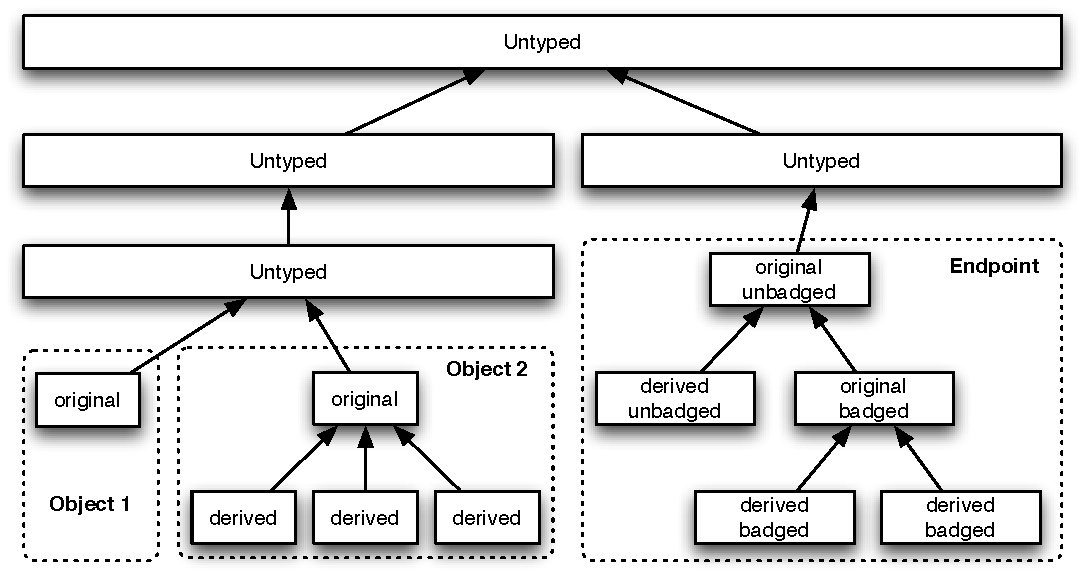
\includegraphics[width=0.8\textwidth]{figs/CDT}
  \end{center}
  \caption{Example capability derivation tree.}\label{fig:CDT}
\end{figure}

\autoref{fig:CDT} shows an example capability derivation tree that
illustrates a standard scenario: the top level is a large untyped
capability, the second level splits this capability into two regions
covered by their own untyped caps, both are children of the first
level.  The third level on the left is a copy of the level 2 untyped
capability.  Untyped capabilities when copied always create children,
never siblings.  In this scenario, the untyped capability was typed
into two separate objects, creating two capabilities on level 4, both
are the original capability to the respective object, both are
children of the untyped capability they were created from.

Ordinary original capabilities can have one level of derived
capabilities.  Further copies of these derived capabilities will
create siblings, in this case remaining on level 5. There is an
exception to this scheme for \obj{Endpoint} and \obj{Notification} capabilities --- they support an
additional layer of depth though \emph{badging}.
The original \obj{Endpoint} or \obj{Notification} capability will be unbadged. Using
the mint method, a copy of the capability with a specific \emph{badge} can be
created (see \autoref{s:ep-badge}, \autoref{s:notif-badge}). This new, badged capability to the same object is treated as
an original capability (the ``original badged endpoint capability'')
and supports one level of derived children like other capabilities.


\section{Deletion and Revocation}
\label{s:cspace-revoke}

Capabilities in seL4 can be deleted and revoked. Both methods
primarily affect capabilities, but they can have side effects on
objects in the system where the deletion or revocation results in the
destruction of the last capability to an object.

As described above, \apifunc{seL4\_CNode\_Delete}{cnode_delete} will
remove a capability from the specified CNode slot. Usually, this is
all that happens. If, however, it was the last typed capability to an
object, this object will now be destroyed by the kernel, cleaning up
all remaining in-kernel references and preparing the memory for
re-use.

If the object to be destroyed was a capability container, i.e.\ a TCB
or CNode, the destruction process will delete each capability held in
the container, prior to destroying the container. This may result in
the destruction of further objects if the contained capabilities are
the last capabilities.\footnote{The recursion is limited as if the last
capability to a CNode is found within the container, the found CNode
is not destroyed. Instead, the found CNode is made unreachable by
moving the capability pointing to the found CNode into the found cnode
itself, by swapping the capability with the first capability in the
found cnode, and then trying to delete the swapped capability
instead. This breaks the recursion.

The result of this approach is that deleting the last cap to the root
CNode of a CSpace does not recursively delete the entire
CSpace. Instead, it deletes the root CNode, and the branches of the
tree become unreachable, potentially including the deleting of some of
the unreachable CNode's caps to make space for the self-referring
capability. The practical consequence of this approach is that CSpace
deletion requires user-level to delete the tree leaf first if
unreachable CNodes are to be avoided. Alternatively, any resulting
unreachable CNodes can be cleaned up via revoking a covering untyped
capability, however this latter approach may be more complex to
arrange by construction at user-level.}

The \apifunc{seL4\_CNode\_Revoke}{cnode_revoke} method will
\apifunc{seL4\_CNode\_Delete}{cnode_delete} all CDT children of the
specified capability, but will leave the capability itself intact. If
any of the revoked child capabilities were the last capabilities to an
object, the appropriate destroy operation is triggered.

Note: \apifunc{seL4\_CNode\_Revoke}{cnode_revoke} may only partially
complete in two specific circumstances. The first being where a
CNode containing the last capability to the TCB of the thread
performing the revoke (or the last capability to the TCB itself) is
deleted as a result of the revoke. In this case the thread performing
the revoke is destroyed during the revoke and the revoke does not
complete. The second circumstance is where the storage containing the
capability that is the target of the revoke is deleted as a result of
the revoke. In this case, the authority to perform the revoke is
removed during the operation and the operation stops part way
through. Both these scenarios can be and should be avoided at
user-level by construction.

Note that for page tables and page directories
\apifunc{seL4\_CNode\_Revoke}{cnode_revoke} will not revoke frame
capabilities mapped into the address space.  They will only be
unmapped from the space.


\section{CSpace Addressing}
\label{s:cspace-addressing}

When performing a system call, a thread specifies to the kernel the
capability to be invoked by giving an address in its CSpace. This
address refers to the specific slot in the caller's CSpace that
contains the capability to be invoked.

CSpaces are designed to permit sparsity, and the process of looking-up
a capability address must be efficient. Therefore, CSpaces are
implemented as \emph{guarded page tables}.
% FIXME: need a references to justify the above decision

As explained earlier, a CSpace is a directed graph of \obj{CNode}
objects, and each \obj{CNode} is a table of slots, where each slot can
either be empty, or contain a capability, which may refer to another \obj{CNode}.
Recall from \autoref{s:sel4_internals} that the number of slots in a \obj{CNode}
must be a power of two. A \obj{CNode} is said to have a \emph{radix}, which is
the power to which two is raised in its size. That is, if a \obj{CNode} has
$2^k$ slots, its radix would be $k$.
The kernel stores a capability to the root \obj{CNode} of each thread's
CSpace in the thread's TCB. Conceptually, a \obj{CNode} capability
stores not only a reference to the \obj{CNode} to which it refers, but
also carries a \emph{guard} value, explained in
\autoref{sec:cap_address_lookup}.

\subsection{Capability Address Lookup}
\label{sec:cap_address_lookup}
Like a virtual memory address, a capability address is simply an
integer. Rather than referring to a location of physical memory (as
does a virtual memory address), a capability address refers to a
capability slot.  When looking up a capability address presented by a
userspace thread, the kernel first consults the \obj{CNode} capability
in the thread's TCB that defines the root of the thread's CSpace. It
then compares that \obj{CNode}'s \emph{guard} value against the most
significant bits of the capability address.  If the two values are
different, lookup fails. Otherwise, the kernel then uses the next
most-significant \emph{radix} bits of the capability address as an
index into the \obj{CNode} to which the \obj{CNode} capability
refers. The slot~$s$ identified by these next \emph{radix} bits might
contain another \obj{CNode} capability or contain something else
(including nothing).  If $s$ contains a \obj{CNode} capability~$c$ and
there are remaining bits (following the \emph{radix} bits) in the
capability address that have yet to be translated, the lookup process
repeats, starting from the \obj{CNode} capability~$c$ and using these
remaining bits of the capability address. Otherwise, the lookup
process terminates successfully; the capability address in question
refers to the capability slot~$s$.

\begin{figure}[tb]
    \begin{center}
        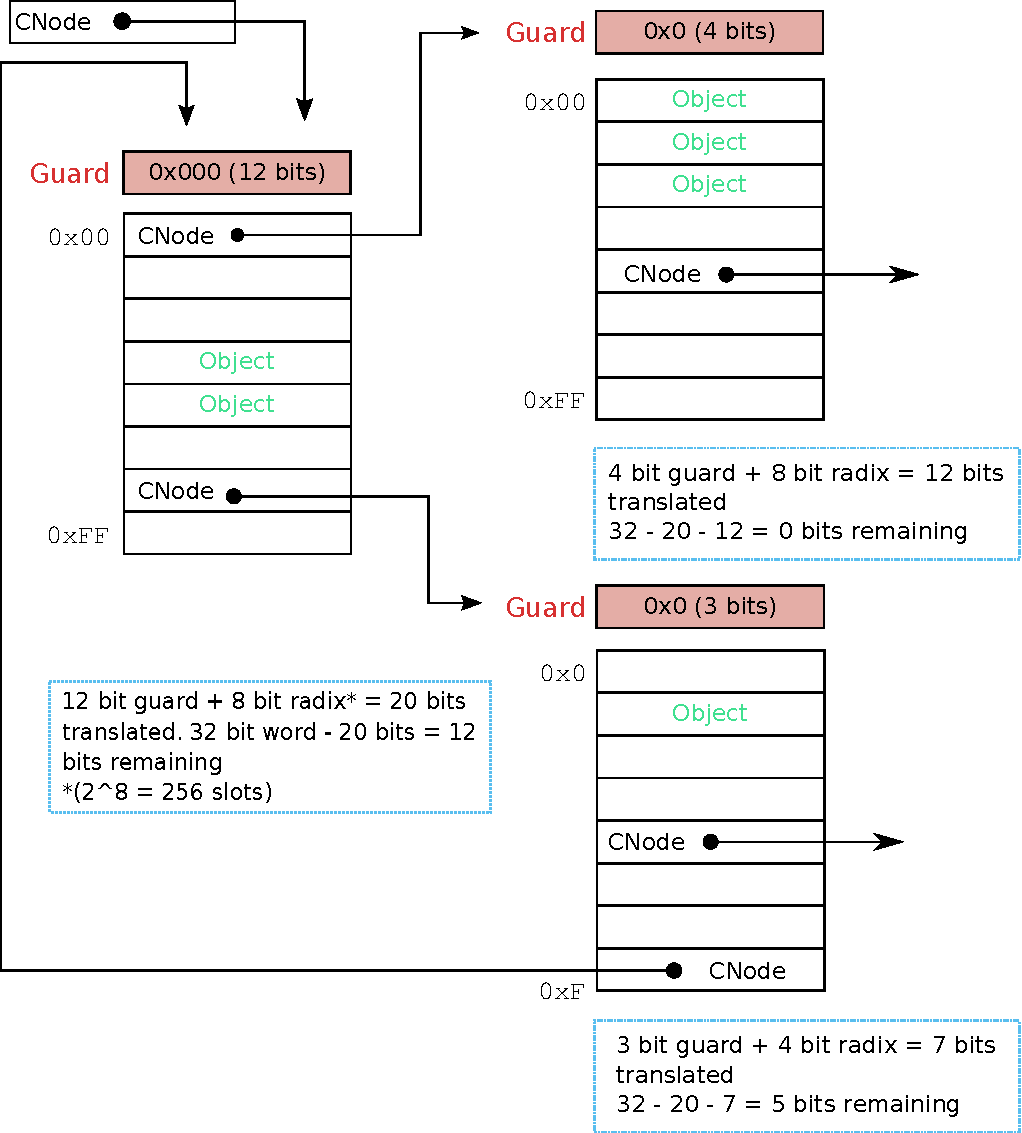
\includegraphics[scale=0.5]{figs/fig1-4.pdf}
        \caption{An example CSpace demonstrating object references at
          all levels, various guard and radix sizes and internal CNode
          references.}
        \label{fig1.4}
    \end{center}
\end{figure}

Figure \ref{fig1.4} demonstrates a valid CSpace with the following
features:
\begin{itemize}
\item a top level CNode object with a 12-bit guard set to 0x000 and
  256 slots;
\item a top level CNode with direct object references;
\item a top level CNode with two second-level CNode references;
\item second level CNodes with different guards and slot counts;
\item a second level CNode that contains a reference to a top level
  CNode;
\item a second level CNode that contains a reference to another CNode
  where there are some bits remaining to be translated;
\item a second level CNode that contains a reference to another CNode
  where there are no bits remaining to be translated; and
\item object references in the second level CNodes.
\end{itemize}

It should be noted that \autoref{fig1.4} demonstrates only what is
possible, not what is usually practical. Although the example CSpace is legal,
it would be reasonably difficult to work with due to the small number
of slots and the circular references within it.


\subsection{Addressing Capabilities}
\label{sec:cap_addressing}

A capability address is stored in a CPointer (abbreviated CPtr), which
is an unsigned integer variable. Capabilities are addressed in
accordance with the translation algorithm described above.  Two
special cases involve addressing \obj{CNode} capabilities themselves
and addressing a range of capability slots.

Recall that the translation algorithm described above will traverse
\obj{CNode} capabilities while there are address bits remaining to be
translated. Therefore, in order to address a capability which may be
a \obj{CNode} capability, the user must supply not only a capability
address but also specify the maximum number of bits of the capability
address that are to be translated, called the \emph{depth limit}.
When a CPointer is paired with depth limit \textit{depth}, only its
\textit{depth} least significant bits are used in translation.

Certain methods, such as
\apifunc{seL4\_Untyped\_Retype}{untyped_retype}, require the user to
provide a range of capability slots. This is done by providing a base
capability address, which refers to the first slot in the range,
together with a window size parameter, specifying the number of slots
(with consecutive addresses, following the base slot) in the range.


\autoref{fig2.1} depicts an example CSpace. In order to illustrate
these ideas, we determine the address of each of the 10 capabilities
in this CSpace.

\begin{figure}[tb]
  \begin{center}
    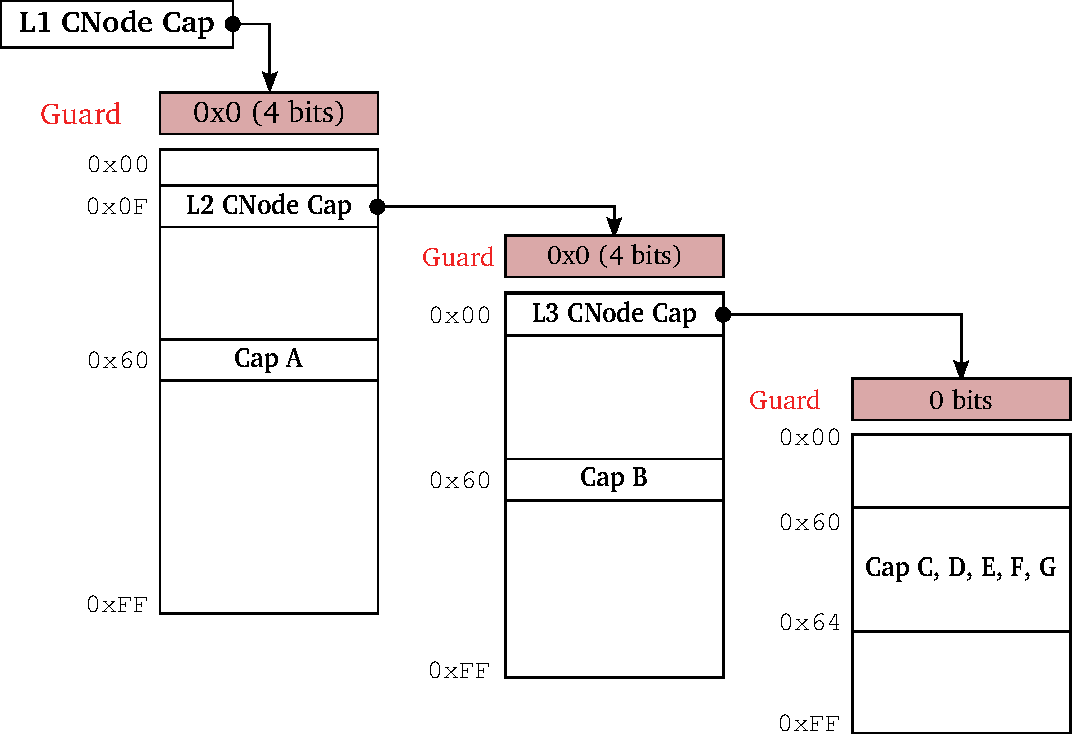
\includegraphics[scale=0.5]{figs/fig2-1.pdf}
    \caption{An arbitrary CSpace layout.}
    \label{fig2.1}
  \end{center}
\end{figure}


\begin{description}
\item[Cap A.] The first CNode has a 4-bit guard set to 0x0, and an
  8-bit radix. Cap A resides in slot 0x60 so, provided that it is not
  a \obj{CNode} capability, it may be referred to by any address of
  the form 0x060\textit{nnnnn} (where \textit{nnnnn} is any sequence
  of 5 hexadecimal digits, because the translation process terminates
  after translating the first 12 bits of the address). For simplicity,
  we usually set unused address bits to 0, which in this case yields
  the address 0x06000000.

\item[Cap B.] Again, the first CNode has a 4-bit guard set to 0x0, and
  an 8-bit radix. The second CNode is reached via the L2 CNode Cap.
  It also has a 4-bit guard of 0x0 and Cap B resides at index
  0x60. Hence, Cap B's address is 0x00F06000.  Translation of this
  address terminates after the first 24 bits.

\item[Cap C.] This capability is addressed via both CNodes. The third
  CNode is reached via the L3 CNode Cap, which resides at index 0x00
  of the second CNode. The third CNode has no guard and Cap C is at
  index 0x60.  Hence, its address is 0x00F00060. Translation of this
  address leaves 0 bits untranslated.

\item[Caps C--G.] This range of capability slots is addressed by
  providing a base address (which refers to the slot containing Cap C)
  of 0x00F00060 and a window size of 5.

\item[L2 CNode Cap.] Recall that to address a \obj{CNode} capability,
  the user must supply not only a capability address but also specify
  the depth limit, which is the maximum number of bits to be
  translated.  L2 CNode Cap resides at offset 0x0F of the first CNode,
  which has a 4-bit guard of 0x0.  Hence, it may be referred to by any
  address of the form 0x\textit{nnnnn}00F with a depth limit of 12
  bits, where \textit{nnnnn} is any sequence of 5 hexadecimal digits.

\item[L3 CNode Cap.] This capability resides at index 0x00 of the
  second CNode, which is reached by the L2 CNode Cap. The second CNode
  has a 4-bit guard of 0x0. Hence, the capability may be referred to
  by any address of the form 0x\textit{nn}00F000 with a depth limit of
  24 bits, where \textit{nn} is any sequence of 2 hexadecimal digits.
\end{description}

In summary, to refer to any capability (or slot) in a CSpace, the user
must supply its address. When the capability might be a CNode, the
user must also supply a depth limit.  To specify a range of capability
slots, the user supplies a starting address and a window size.

\section{Lookup Failure Description}
\label{sec:lookup_fail_desc}

When a capability lookup fails, a description of the failure is given
to either the calling thread or the thread's exception handler in its
IPC buffer.  The format of the description is always the same but may
occur at varying offsets in the IPC buffer depending on how the error
occurred.  The description format is explained below.  The first word
indicates the type of lookup failure and the meaning of later words
depend on this.

\subsection{Invalid Root}

A CSpace CPtr root (within which a capability was to be looked up)
is invalid. For example, the capability is not a \obj{CNode} cap.\\  \\

\begin{tabularx}{\textwidth}{XX}
  \toprule
  Data & Meaning \\
  \midrule
  \ipcbloc{Offset + 0} & \enummem{seL4\_InvalidRoot} \\
  \bottomrule
\end{tabularx}

\subsection{Missing Capability}

A capability required for an invocation is not present or does not
have sufficient rights. \\ \\

\begin{tabularx}{\textwidth}{XX}
  \toprule
  Data & Meaning \\
  \midrule
  \ipcbloc{Offset + 0} & \enummem{seL4\_MissingCapability} \\
    \ipcbloc{Offset + seL4\_CapFault\_BitsLeft} & Bits left \\
  \bottomrule
\end{tabularx}

\subsection{Depth Mismatch}

When resolving a capability, a CNode was traversed that resolved more
bits than was left to decode in the CPtr or a non-CNode capability was
encountered while there were still bits remaining to be looked up. \\ \\

\begin{tabularx}{\textwidth}{XX}
  \toprule
  Data & Meaning \\
  \midrule
  \ipcbloc{Offset + 0} & \enummem{seL4\_DepthMismatch} \\
  \ipcbloc{Offset + seL4\_CapFault\_BitsLeft} & Bits of CPtr remaining to decode \\
  \ipcbloc{Offset + seL4\_CapFault\_DepthMismatch\_BitsFound} & Bits that the current CNode being traversed resolved \\
  \bottomrule
\end{tabularx}

\subsection{Guard Mismatch}

When resolving a capability, a CNode was traversed with a guard size
larger than the number of bits remaining or the CNode's guard did not
match the next bits of the CPtr being resolved. \\ \\

\begin{tabularx}{\textwidth}{XX}
  \toprule
  Data & Meaning \\
  \midrule
  \ipcbloc{Offset + 0} & \enummem{seL4\_GuardMismatch} \\
    \ipcbloc{Offset + seL4\_CapFault\_BitsLeft} & Bits of CPtr remaining to decode \\
  \ipcbloc{Offset + seL4\_CapFault\_GuardMismatch\_GuardFound} & The CNode's guard \\
  \ipcbloc{Offset + seL4\_CapFault\_GuardMismatch\_BitsFound} & The CNode's guard size \\
  \bottomrule
\end{tabularx}



  %
% Copyright 2014, General Dynamics C4 Systems
%
% SPDX-License-Identifier: GPL-2.0-only
%

\chapter{\label{ch:ipc}Message Passing (IPC)}

The seL4 microkernel provides a message-passing IPC mechanism for communication
between threads. The same mechanism is also used for communication with
kernel-provided services. Messages are sent by invoking a capability to a
kernel object. Messages sent to \obj{Endpoint}s are destined for other
threads, while messages sent to other objects are processed by the kernel. This
chapter describes the common message format, endpoints,
and how they can be used for communication between applications.

\section{Message Registers}
\label{sec:messageinfo}

Each message contains a number of message words and optionally a number of
capabilities.
The message words are sent to or received from a thread by placing them in its \emph{message registers}.
The message registers are numbered and the first few message registers are implemented
using physical CPU registers, while the rest are backed by a fixed region of
memory called the \emph{IPC buffer}.
The reason for this design is efficiency:
very short messages need not use the memory.
The IPC buffer is assigned to the calling thread (see \autoref{sec:threads} and \autoref{api:tcb_setipcbuffer}).
%FIXME: seL4_TCB_SetIPCBuffer is only mentioned in the API reference!

Every IPC message also has a tag (structure \texttt{seL4\_MessageInfo\_t}).  The
tag consists of four fields: the label, message length, number of capabilities
(the \texttt{extraCaps} field) and the \texttt{capsUnwrapped} field.  The
message length and number of capabilities determine either the number of
message registers and capabilities that the sending thread wishes to transfer,
or the number of message registers and capabilities that were actually
transferred. The label is not interpreted by the
kernel and is passed unmodified as the first data payload of the message. The
label may, for example, be used to specify a requested operation. The
\texttt{capsUnwrapped} field is used only on the receive side, to indicate the
manner in which capabilities were received. It is described in
\autoref{sec:cap-transfer}.

% FIXME: a little too low-level, perhaps?

\newcommand{\ipcparam}[4]{\texttt{#1} \emph{#2}&\texttt{#3}&#4\\ }
\begin{table}[htb]
    \begin{center}
    \begin{tabularx}{\textwidth}{p{0.28\textwidth}p{0.18\textwidth}X}
      \toprule
      \textbf{Type} & \textbf{Name} & \textbf{Description} \\
      \midrule
        \ipcparam{seL4\_MessageInfo\_t}{}{tag}{Message tag}
        \ipcparam{seL4\_Word[]}{}{msg}{Message contents}
        \ipcparam{seL4\_Word}{}{userData}{Base address of the structure, used by
        supporting user libraries}
        \ipcparam{seL4\_CPtr[]}{(in)}{caps}{Capabilities to transfer}
        \ipcparam{seL4\_CapData\_t[]}{(out)}{badges}{Badges for
        endpoint capabilities received}
        \ipcparam{seL4\_CPtr}{}{receiveCNode}{CPtr to a CNode from which to
        find
        the receive slot}
        \ipcparam{seL4\_CPtr}{}{receiveIndex}{CPtr to the receive slot
        relative to \texttt{receiveCNode}}
        \ipcparam{seL4\_Word}{}{receiveDepth}{Number of bits of
        \texttt{receiveIndex} to
        use}
        \bottomrule
      \end{tabularx}
    \caption{\label{tbl:ipcbuffer}Fields of the
      \texttt{seL4\_IPCBuffer} structure.  Note that
      \texttt{badges} and \texttt{caps} use the same area of memory in
      the structure.}
    \end{center}
\end{table}

The kernel assumes that the IPC buffer contains a structure of type
\texttt{seL4\_IPCBuffer} as defined in \autoref{tbl:ipcbuffer}. The
kernel uses as many physical registers as possible to transfer IPC
messages. When more arguments are transferred than physical message
registers are available, the kernel begins using the IPC buffer's
\texttt{msg} field to transfer arguments. However, it leaves room in
this array for the physical message registers. For example, if an IPC
transfer or kernel object invocation required
4 message registers (and there are only 2 physical message registers
available on this architecture) then arguments 1 and 2 would be
transferred via message registers and arguments 3 and 4 would be in
\texttt{msg[2]} and \texttt{msg[3]}.
This allows the user-level object-invocation stubs to copy the arguments passed in physical registers to
the space left in the \texttt{msg} array if desired.
The situation is similar for the tag field.
There is space for this field in the \texttt{seL4\_IPCBuffer} structure, which the kernel ignores.
User level stubs
may wish to copy the message tag from its CPU register to this field, although
the user level stubs provided with the kernel do not do this.

\section{Endpoints}

\obj{Endpoint}s allow a small amount
of data and capabilities (namely the IPC buffer) to be transferred between two
threads. \obj{Endpoint} objects are invoked directly using the seL4 system calls
described in \autoref{sec:syscalls}.

IPC \obj{Endpoints} uses a rendezvous model and as such is
synchronous and blocking. An \obj{Endpoint} object  may queue
threads either to send or to receive. If no receiver is ready, threads
performing the \apifunc{seL4\_Send}{sel4_send} or \apifunc{seL4\_Call}{sel4_call}
system calls will wait in a queue for the first available receiver. Likewise, if
no sender is ready, threads performing the \apifunc{seL4\_Recv}{sel4_recv}
system call or the second half of \apifunc{seL4\_ReplyRecv}{sel4_replyrecv}
will wait for the first available sender.

Trying to Send or Call without the Write right will fail and return an error. In
the case of Send the error is ignored (the kernel isn't allowed to reply). Thus
there is no way of knowing that a send has failed because of a missing right.
On the other hand calling \apifunc{seL4\_Recv}{sel4_recv} with a endpoint capability that
does not have the Read right will raise a fault, see \autoref{sec:faults}. This is
because otherwise the error message would be indistinguishable from a normal
message received from another thread via the endpoint.

\subsection{Endpoint Badges\label{s:ep-badge}}
\label{sec:ep-badges}

Endpoint capabilities may be \emph{minted} to
create a new endpoint capability with a \emph{badge} attached to it, a data
word chosen by the invoker of the \emph{mint} operation. When a message is sent to an endpoint using a badged
capability, the badge is transferred to the receiving thread's
\texttt{badge} register.

An endpoint capability with a zero badge is said to be \emph{unbadged}.
Such a capability can be badged with the \apifunc{seL4\_CNode\_Mint}{cnode_mint}
invocation on the \obj{CNode} containing the capability. Endpoint
capabilities with badges cannot be unbadged, rebadged or used to create
child capabilities with different badges.

On 32-bit platforms, only the low 28 bits of the badge are available for use.
The kernel will silently ignore any usage of the high 4 bits.
On 64-bit platforms, 64 bits are available for badges.

\subsection{Capability Transfer}
\label{sec:cap-transfer}

Messages may contain capabilities, which will be copied to the
receiver, provided that the endpoint capability
invoked by the sending thread has Grant rights. An attempt to send
capabilities using an endpoint capability without the Grant right will
result in a transfer of the raw message, without any capability transfer.

Capabilities to be sent in a message are specified in the sending thread's
IPC buffer in the \texttt{caps} field. Each entry in that array is interpreted
as a CPtr in the sending thread's capability space. The number of capabilities
to send is specified in the \texttt{extraCaps} field of the message tag.

The receiver specifies the slot
in which it is willing to receive a capability, with three fields within the IPC buffer: \texttt{receiveCNode}, \texttt{receiveIndex} and \texttt{receiveDepth}.
These fields specify the root CNode, capability address and number of bits to resolve, respectively, to find
the slot in which to put the capability. Capability
addressing is described in \autoref{sec:cap_addressing}.

Note that receiving threads may specify only one receive slot, whereas a
sending thread may include multiple capabilities in the message. Messages
containing more than one capability may be interpreted by kernel objects. They
may also be sent to receiving threads in the case where some of the extra
capabilities in the message can be \emph{unwrapped}.

If the n-th capability in the message refers to the endpoint through
which the message is sent, the capability is \emph{unwrapped}: its badge is placed into
the n-th
position of the receiver's badges array, and the kernel sets the n-th bit (counting from the
least significant) in the \texttt{capsUnwrapped} field of the message
tag. The capability itself is not transferred, so the receive slot may be used
for another capability.

A capability that is not unwrapped is transferred by copying it from the
sender's CNode slot to the receiver's CNode slot. The sender retains access
to the sent capability.

If a receiver gets a message whose tag has an \texttt{extraCaps} of 2 and a
\texttt{capsUnwrapped} of 2, then the first capability in the message was
transferred to the specified receive slot and the second capability was
unwrapped, placing its badge in \texttt{badges[1]}. There may have been a
third capability in the sender's message which could not be unwrapped.

\subsection{Errors}

Errors in capability transfers can occur at two places: in the send
phase or in the receive phase. In the send phase, all capabilities that
the caller is attempting to send are looked up to ensure that they exist
before the send is initiated in the kernel. If the lookup fails for any
reason, \apifunc{seL4\_Send}{sel4_send} and \apifunc{seL4\_Call}{sel4_call} system calls immediately abort and
no IPC or capability transfer takes place. The system call will return
a lookup failure error as described in \autoref{sec:errors}.

In the receive phase, seL4 transfers capabilities in the order they
are found in the sending thread's IPC buffer \texttt{caps} array
and terminates as soon as an error is encountered. Possible error
conditions are:

\begin{itemize}
    \item A source capability cannot be looked up. Although the presence
    of the source capabilities is checked when the sending thread
    performs the send system call, this error may still occur. The sending
    thread may have been blocked on the endpoint for some time before it
    was paired with a receiving thread. During this time, its
    CSpace may have changed and the source capability pointers may
    no longer be valid.

    \item The destination slot cannot be looked up. Unlike the send system call,
    the \apifunc{seL4\_Recv}{sel4_recv} system call does not check that the
    destination slot exists and is empty before it initiates the receive
    operation. Hence, the \apifunc{seL4\_Recv}{sel4_recv} system call will not
    fail with an error if the destination slot is invalid and will instead
    transfer badged capabilities until an attempt to save a capability to the
    destination slot is made.

    \item The capability being transferred cannot be derived. See
    \autoref{sec:cap_derivation} for details.
\end{itemize}

An error will not void the entire transfer, it will just end it
prematurely. The capabilities processed before the failure are still
transferred and the \texttt{extraCaps} field in the receiver's IPC
buffer is set to the number of capabilities transferred up to failure.
No error message will be returned to the receiving thread in any of the
above cases.

\subsection{Calling and Replying}
\label{sec:ep-cal}

As explained in \autoref{sec:sys_call}, when the user calls
\apifunc{seL4\_Call}{sel4_call} on an endpoint capability,
some specific actions are taken. First a call will do exactly the same action as
a normal \apifunc{seL4\_Send}{sel4_send}. Then after the rendezvous and all the
normal IPC procedure happened, instead of returning directly to the caller,
\apifunc{seL4\_Call}{sel4_call} will check if either Grant or GrantReply are
present on the invoked endpoint capability:

\begin{itemize}
\item If this is not the case, the caller thread is suspended as if
  \apifunc{seL4\_TCB\_Suspend}{tcb_suspend} was called on it. The send part of
  the call would still have been performed as usual.
\item If this is the case. A reply capability is set in a specific slot of the
  receiver TCB. The Grant right of that reply capability is set by copying the Grant
  right of the endpoint capability invoked by the receiver in
  \apifunc{seL4\_Recv}{sel4_recv}.
  Then, the caller thread is blocked waiting for the reply.
  \end{itemize}

A reply capability points directly to the caller thread and once the call has
been performed is completely unrelated to the original \obj{Endpoint}. Even if
the latter was destroyed, the reply capability would still exist and point to
the caller who would still be waiting for a reply.

The generated reply capability can then be either invoked in place (in the
specific TCB slot) with the \apifunc{seL4\_Reply}{sel4_reply} or saved to an
addressable slot using \apifunc{seL4\_CNode\_SaveCaller}{cnode_savecaller} to be
invoked later with \apifunc{seL4\_Send}{sel4_send}. The specific slot cannot be
directly addressed with any CPtr as it is not part of any CSpace.

A reply capability is invoked in the same way as a normal send on a
\obj{Endpoint}. A reply capability has implicitly the Write right, so the
message will always go through. Transferring caps in the reply can only happen
if the reply capability has the Grant right and is done in exactly the same way
as in a normal IPC transfer as described in \autoref{sec:cap-transfer}.

The main difference with a normal endpoint transfer is that the kernel guarantees
that invoking a reply capability cannot block: If you own a reply capability,
then the thread it points to is waiting for a reply. However a reply capability
is a non-owning reference, contrary to all the other capabilities. That means that
if the caller thread is destroyed or modified in any way that would render
a reply impossible (for example being suspended with
\apifunc{seL4\_TCB\_Suspend}{tcb_suspend}), the kernel would immediately destroy
the reply capability.

Once the reply capability has been invoked, the caller receives the message as if
it has been performing a \apifunc{seL4\_Recv}{sel4_recv} and just received the
message. In particular, it starts running again.

The \apifunc{seL4\_Call}{sel4_call} operation exists not only for
efficiency reasons (combining two operations into a single system
call). It differs from
\apifunc{seL4\_Send}{sel4_send} immediately followed by
\apifunc{seL4\_Recv}{sel4_recv} in ways that allow certain system setup to work
much more efficiently with much less setup than with a traditional setup.
In particular, it is guaranteed that the reply received by the caller comes from
the thread that received the call without having to check any kind of badge.

  %
% Copyright 2014, General Dynamics C4 Systems
%
% SPDX-License-Identifier: GPL-2.0-only
%

\chapter{\label{ch:notifications}Notifications}

Notifications are a simple, non-blocking signalling mechanism that
logically represents a set of binary semaphores.

\section{Notification Objects}

A \obj{Notification} object contains a single data word, called the
\emph{notification word}. Such an object supports two operations:
\apifunc{seL4\_Signal}{sel4_signal} and
\apifunc{seL4\_Wait}{sel4_wait}.

\obj{Notification} capabilities can be badged, using
\apifunc{seL4\_CNode\_Mint}{cnode_mint}, just like \obj{Endpoint}
capabilities (see \autoref{sec:ep-badges}). As with \obj{Endpoint}
capabilities, badged \obj{Notification} capabilities cannot be
unbadged, rebadged or used to create child capabilities with
different badges. \label{s:notif-badge}

\section{Signalling, Polling and Waiting}

The \apifunc{seL4\_Signal}{sel4_signal} method updates the
notification word by bit-wise \texttt{or}-ing it with the \emph{badge}
of the invoked notification capability. It also unblocks the first
thread waiting on the notification (if any). As such,
\apifunc{seL4\_Signal}{sel4_signal} works like concurrently signalling
multiple semaphores (those indicated by the bits set in the badge).
If the signal sender capability was unbadged or 0-badged, the operation degrades
to just waking up the first thread waiting on the notification (also see below).

The \apifunc{seL4\_Wait}{sel4_wait} method works similarly to a
select-style wait on the set of semaphores: If the notification word is
zero at the time \apifunc{seL4\_Wait}{sel4_wait} is called, the
invoker blocks. Else, the call returns immediately, setting the
notification word to zero and returning to the invoker the previous
notification-word value.

The \apifunc{seL4\_Poll}{sel4_poll} is the same as \apifunc{seL4\_Wait}{sel4_wait}, except if
no signals are pending (the notification word is 0) the call will return immediately
without blocking.

If threads are waiting on the \obj{Notification} object at the time
\apifunc{seL4\_Signal}{sel4_signal} is invoked, the first queued thread
receives the notification. All other threads keep waiting until the
next time the notification is signalled.

\section{Binding Notifications}
\label{sec:notification-binding}

\obj{Notification} objects and \obj{TCB}s can be bound together in a 1-to-1 relationship
through the \apifunc{seL4\_TCB\_BindNotification}{tcb_bindnotification} invocation. When a
\obj{Notification} is bound to a \obj{TCB}, signals to that notification object
will be delivered even if the thread is receiving from an IPC
endpoint. To distinguish whether the received message was a notification
or an IPC, developers should check the badge value. By reserving a
specific badge (or range of badges) for capabilities to the bound
notification --- distinct from endpoint badges --- the
message source can be determined.

Once a notification has been bound, the only thread that may perform
\apifunc{seL4\_Wait}{sel4_wait} on the notification is the bound thread.

  %
% Copyright 2014, General Dynamics C4 Systems
%
% SPDX-License-Identifier: GPL-2.0-only
%

\chapter{\label{ch:threads}Threads and Execution}

\section{Threads}
\label{sec:threads}


seL4 provides threads to represent an execution context. On MCS configurations of
the kernel, scheduling contexts are used to manage processor time. Without MCS, processor
time is also represented by the thread abstraction.
A thread is represented in seL4 by its thread control block
object (\obj{TCB}).

With MCS, a scheduling context is represented by a scheduling context object
(\obj{SCO}), and threads cannot run unless they are bound to, or receive a
scheduling context.

\subsection{Thread control blocks}

Each \obj{TCB} has an associated CSpace (see
\autoref{ch:cspace}) and VSpace (see \autoref{ch:vspace}) which
may be shared with other threads. A \obj{TCB} may also have an IPC buffer
(see  \autoref{ch:ipc}), which is used to pass extra arguments during IPC
or kernel object invocation that do not fit in the architecture-defined message
registers. While it is not compulsory that a thread has an IPC buffer,
it will not be able to perform most kernel invocations, as they require
cap transfer.
Each thread belongs to exactly one security domain (see
\autoref{sec:domains}).
%FIXME: there is much more information held in the TCB!

\subsection{Thread Creation}
\label{sec:thread_creation}

Like other objects, \obj{TCB}s are created with the
\apifunc{seL4\_Untyped\_Retype}{untyped_retype} method (see
\autoref{sec:kernmemalloc}). A newly created thread is initially inactive. It
is configured by setting its CSpace and VSpace with the
\apifunc{seL4\_TCB\_SetSpace}{tcb_setspace}
or \apifunc{seL4\_TCB\_Configure}{tcb_configure} methods and then calling
\apifunc{seL4\_TCB\_WriteRegisters}{tcb_writeregisters} with an initial stack pointer and instruction
pointer. The thread can then be activated either by setting the
\texttt{resume\_target} parameter in the \apifunc{seL4\_TCB\_WriteRegisters}{tcb_writeregisters} invocation to true
or by separately calling the \apifunc{seL4\_TCB\_Resume}{tcb_resume} method. Both of these methods
place the thread in a runnable state.

In non-MCS configurations of the kernel, this will result in the thread immediately being added to
the scheduler. On the MCS kernel, the thread will only begin running if it has a
scheduling context object.

In a SMP configuration of the kernel, the thread will resume on the node
corresponding to the affinity of the thread. For non-MCS configurations, the
default thread affinity is the node the thread's \obj{TCB} object was created
on, and \apifunc{seL4\_TCB\_SetAffinity}{tcb_setaffinity} can be used to
explicitly set the affinity. On MCS configurations, the affinity is derived
from the scheduling context object (see \autoref{sec:sc_creation}).

\subsection{Thread Deactivation}
\label{sec:thread_deactivation}

The \apifunc{seL4\_TCB\_Suspend}{tcb_suspend} method deactivates a thread.
Suspended threads can later be resumed.
Their suspended state can be retrieved with the
\apifunc{seL4\_TCB\_ReadRegisters}{tcb_readregisters} and
\apifunc{seL4\_TCB\_CopyRegisters}{tcb_copyregisters} methods.
They can also be reconfigured and
reused or left suspended indefinitely if not needed. Threads will be
automatically suspended when the last capability to their \obj{TCB} is
deleted.
% an example of which is demonstrated in \nameref{ex:second_thread}.

\subsection{Affinity}
\label{sec:thread_affinity}

It is architecture and platform specific, how an affinity value maps to a
specific node (core, hart) on a specific platform. There is no guarantee that
affinity values are compatible across different platforms.


\subsection{Scheduling}
\label{sec:sched}

seL4 uses a preemptive, tickless scheduler with 256 priority levels (0 --- 255).  All threads have
a maximum controlled priority (MCP) and a priority, the latter being the effective priority of the
thread.
When a thread modifies another thread's priority (including itself) it must provide a
thread capability from which to use the MCP from. Threads can only set priorities and MCPs
to be less than or equal to the provided thread's MCP.
The initial task starts with an MCP and priority as the highest priority in the system (\texttt{seL4\_MaxPrio}).
Thread priority and MCP can be
set with \apifunc{seL4\_TCB\_SetSchedParams}{tcb_setschedparams} and
\apifunc{seL4\_TCB\_SetPriority}{tcb_setpriority},
\apifunc{seL4\_TCB\_SetMCPriority}{tcb_setmcpriority} methods.


Of threads eligible for scheduling, the highest priority thread in a runnable state is chosen.

Thread priority (structure \texttt{seL4\_PrioProps\_t}) consists of two values as follows:

\begin{description} \item[Priority] the priority a thread will be scheduled with.  \item[Maximum
controlled priority (MCP)] the highest priority a thread can set itself or another thread to.
\end{description}

\subsection{MCS Scheduling}

This section only applies to configurations with MCS enabled, where threads must have
a scheduling context object available in order to be admitted to the scheduler.

\subsection{Scheduling Contexts}
\label{sec:scheduling_contexts}

Access to CPU execution time is controlled through scheduling context objects.
Scheduling contexts are configured with a tuple of
\textit{budget}$(b)$ and \textit{period} $(p)$, both in microseconds, set by
\apifunc{seL4\_SchedControl\_Configure\_Flags}{schedcontrol_configureflags} (see \autoref{sec:sc_creation}).
The tuple $(b, p)$ forms an upper bound on the thread's execution -- the kernel will not permit a
thread to run for more than $b$ out of every $p$ microseconds. However, $\frac{b}{p}$ does not
represent a lower bound on execution, as a thread must have the highest or equal highest priority
of all runnable threads to be guaranteed to be scheduled at all, and the kernel does not conduct
an admission test. As a result the set of all parameters is not necessarily schedulable. If
multiple threads have budgets available concurrently they are scheduled first-in first-out, and
round-robin scheduling is applied once the budget is expired.

A scheduling context that is eligible to be picked by the scheduler, i.e has budget available, is
referred to as \emph{active}.  Budget charging and replenishment rules are different for round-robin
and sporadic threads.  For round-robin threads, the budget is charged each time the current node's
scheduling context is changed, until it is depleted and then refilled immediately.

Threads where $b == p$ are treated as round robin threads, where $b$ acts as a timeslice.
Otherwise the kernel uses \emph{sporadic servers} to enforce temporal isolation, which enforce the
property that $\frac{b}{p}$ cannot be exceeded for all possible $p$.
In theory, sporadic servers provide temporal isolation -- preventing threads from exceeding their allocated budget -- by using the following algorithm:

\begin{itemize}
\item When a thread starts executing at current time $T$, record $T_{s}$
\item When a thread stops executing (blocks or is preempted), schedule a replenishment at $T_{s} + p$ for the
amount of time consumed ($T - T_{s}$) and subtract that from the current replenishment being used.
\end{itemize}

seL4 implements this algorithm by maintaining an ordered list of sporadic replenishments --
\texttt{refills} for brevity -- in each scheduling context. Each replenishment contains a tuple
of the time it is eligible for use (\emph{rTime}) and the amount that replenishment is for
(\texttt{rAmount}).
While a thread is executing, it constantly drains the budget from the \texttt{rAmount} at the head of the
replenishment list. If the \texttt{rTime} is in the future, the thread bound to that
scheduling context is placed in a queue of threads waiting for more budget.

Round-robin threads are treated that same as sporadic threads except regarding one aspect: how the
budget is charged. Round-robin threads have two refills only, both of which are always ready to be
used. When a round-robin thread stops executing, budget is moved from the head to the tail
replenishment. Once the head budget is consumed, the thread is removed from the scheduling queue
for its priority and appended at the tail.

Sporadic threads behave differently depending on the amount of replenishments available, which
must be bounded. Developers have two options to configure the size of the replenishment list:

\begin{itemize}
\item The maximum number of refills in a single scheduling context is determined by the size
      of the scheduling context when created by \apifunc{seL4\_Untyped\_Retype}{untyped_retype}.
\item A per scheduling context parameter, \texttt{extra\_refills} that
limits the number of refills for that specific scheduling context. This value is added to the base
value of 2 and is limited by the size of the scheduling context.
\end{itemize}

Threads that have short execution times (e.g interrupt handlers) and are not frequently preempted
should have less refills, while longer running threads with long values of $b$ should have a higher
value. Threads bound to a scheduling context with 0 extra refills will run periodically -- tasks
that use their head replenishment, or call yield, will not be scheduled again until the start of
their next period.

Given the number of replenishments is limited, if a node's SC changes and the outgoing SC does not
have enough space to store the new replenishment, space is created by removing the current
replenishment which can result in preemption if the next replenishment is not yet available.
Scheduling contexts with a higher number of configured refills will consume closer
to their whole budget, as they can be preempted and switch threads more often without filling their
replenishment queue. However, the scheduling overhead will be higher as the replenishment list is
subject to fragmentation.

Whenever a thread is executing it consumes the budget from its current scheduling context.  The
system call \apifunc{seL4\_Yield}{sel4_yield} can be used to sacrifice any remaining budget and
block until the next replenishment is ready to be used.

Threads can be bound to scheduling contexts using \apifunc{seL4\_TCB\_Configure}{tcb_configure} or
\apifunc{seL4\_SchedContext\_Bind}{schedcontext_bind}, both invocations have the same effect
although \apifunc{seL4\_TCB\_Configure}{tcb_configure} allows more thread fields to be set with only
one kernel entry.  When a thread is bound to a scheduling context, if it is in a runnable state and
the scheduling context is active, it will be added to the scheduler.

\subsection{Passive Threads} \label{sec:passive}

Threads can be unbound from a scheduling context with
\apifunc{seL4\_SchedContext\_UnbindObject}{schedcontext_unbindobject}.  This is distinct from
suspending a thread, in that threads that are blocked waiting in an endpoint or notification queue
will remain in the queue and can still receive messages and signals.  However, the unbound thread
will not be schedul\-able again until it receives a scheduling context.  Threads without scheduling
contexts are referred to as \emph{passive} threads, as they cannot execute without the action of
another thread.

\subsection{Scheduling Context Creation} \label{sec:sc_creation}

Like other objects, scheduling contexts are created from untyped memory using
\apifunc{seL4\_UntypedRetype}{untyped_retype}.  On creation, scheduling contexts are empty,
representing 0\% of CPU execution time.  To populate a scheduling context with parameters, one must
invoke the appropriate \obj{SchedControl} capability, which provides access to CPU time management
on a single node.  A scheduling control cap for each node is provided to the initial task at run
time.  Threads run on the node that their scheduling context is configured for.  Scheduling context
parameters can then be set and updated using
\apifunc{seL4\_SchedControl\_ConfigureFlags}{schedcontrol_configureflags}, which allows the budget and period
to be specified along with a bitwise OR'd set of the following flags.

\begin{description}

\item[seL4\_SchedContext\_Sporadic]: constrain the execution time only according to the
sporadic server algorithm rather than to a continuous constant bandwidth.

\end{description}

The kernel does not conduct any schedulability tests, as task admission is left to user-level policy
and can be conducted online or offline, statically or dynamically or not at all.

\subsection{Scheduling Context Donation}

In addition to explicitly binding and removing scheduling contexts through
\apifunc{seL4\_SchedContext\_Bind}{schedcontext_bind} and
\apifunc{seL4\_SchedContext\_UnbindObject}{schedcontext_unbindobject}, scheduling contexts can move
between threads over IPC.  Scheduling contexts are donated implicitly when the system calls
\apifunc{seL4\_Call}{sel4_call} and \apifunc{seL4\_NBSendRecv}{sel4_nbsendrecv} are used to
communicate with a passive thread.  When an active thread invokes an endpoint with
\apifunc{seL4\_Call}{sel4_call} and rendezvous with a passive thread, the active thread's scheduling
context is donated to the passive thread. The generated reply cap ensures that the callee is merely
borrowing the scheduling context: when the reply cap is consumed by a reply message being sent the
scheduling context will be returned to the caller.  If the reply cap is revoked, and the callee
holds the scheduling context, the scheduling context will be returned to the caller.  However, if in
a deep call chain and a reply cap in the middle of the call chain is revoked, such that the callee
does not possess the scheduling context, the thread will be removed from the call chain and the
scheduling context will remain where it is.  If the receiver does not provide a reply object to
track the donation in (i.e uses \apifunc{seL4\_Wait}{sel4_wait} instead of
\apifunc{seL4\_Recv}{sel4_recv} scheduling context donation will not occur but the message will be
delivered. The passive receiver will be set to inactive as it does not have a scheduling context.

Consider an example where thread A calls thread B which calls thread C.  If whilst C holds the
scheduling context, B's reply cap to A is revoked, then the scheduling context will remain with C.
However, a call chain will remain between A and C, such that if C's reply cap is revoked, or
invoked, the scheduling context will return to A.

\apifunc{seL4\_NBSendRecv}{sel4_nbsendrecv} can also result in scheduling context donation.
If the non-blocking send phase of the operation results in message delivery to a passive thread, the
scheduling context will be donated to that passive thread and the thread making the system call becomes passive on the
receiving endpoint in the receive phase.  No reply capability is generated, so there
is no guarantee that the scheduling context will return, which increases book keeping complexity but allows
for data-flow like architectures rather than remote-procedure calls. Note that \apifunc{seL4\_Call}{sel4_call}
does not guarantee the return of a scheduling context: this is an inherently trusted operation as the
server could never reply and return the scheduling context.

Scheduling contexts can also be bound to notification objects using
\apifunc{seL4\_SchedContext\_Bind}{schedcontext_bind} and unbound using
\apifunc{seL4\_SchedContext\_UnbindObject}{schedcontext_unbindobject}.  If a signal is delivered to
a notification object with a passive thread blocked waiting on it, the passive thread will receive
the scheduling context that is bound to the notification object.  The scheduling context is returned
when the thread blocks on the notification object.  This feature allows for passive servers to use
notification binding (See \autoref{sec:notification-binding}).  If a scheduling context is bound to
both a notification object and a thread, the behaviour will be the same as for a passive server:
The scheduling context will be unbound from the thread when it blocks on the bound notification object.
This is useful when launching passive servers or handling timeout exceptions.

Scheduling contexts can be unbound from all objects (notification objects and TCBs that are bound or
have received a scheduling context through donation) using
\apifunc{seL4\_SchedContext\_Unbind}{schedcontext_unbind}.

Passive threads will run on the CPU node that the scheduling context was configured with, and will
be migrated on IPC.

\subsection{Scheduling algorithm} \label{sec:mcs-sched}

Threads are only eligible for scheduling if they have an active scheduling context.
Of threads eligible for scheduling, the highest priority thread in a runnable state is chosen.

Threads of sufficient maximum controlled priority and with possession of the
appropriate scheduling context capability can manipulate the scheduler and
implement user-level schedulers using IPC.

Scheduling contexts provide access to an upper bound on execution CPU time,
however when a thread executes is determined by thread priority.  Consequently,
access to CPU is a function of thread MCPs, scheduling contexts and the
\obj{SchedControl} capability.  The kernel will enforce that threads do not
exceed the budget in their scheduling context for any given period, and that
the highest priority thread will always run, however it is up to the system
designer to make sure the entire system is schedulable.


\subsection{Exceptions}
\label{sec:exceptions}

Each thread has two associated exception-handler endpoints, a \emph{standard}
exception handler and a \emph{timeout} exception handler, where the latter is MCS
only. If the thread causes
an exception, the kernel creates an IPC message with the relevant details and
sends this to the endpoint. This thread can then take the appropriate action.
Fault IPC messages are described in \autoref{sec:faults}.  Standard exception-handler
endpoints can be set with the \apifunc{seL4\_TCB\_SetSpace}{tcb_setspace} or
\apifunc{seL4\_TCB\_SetSchedParams}{tcb_setschedparams} methods while Timeout exception
handlers can be set with \apifunc{seL4\_TCB\_SetTimeoutEndpoint}{tcb_settimeoutendpoint} (MCS only).
With these methods, a
capability address for the exception handler can be associated with a thread.
This address is then used to lookup the handler endpoint, and the capability to
the endpoint is installed into the threads' kernel CNode.  For threads without
an exception handler, a null capability can be used, however the consequences
are different per exception handler type.  Before raising an exception the
handler capability is validated. The kernel does not perform another lookup,
but checks that the capability is an endpoint with the correct rights.

The exception endpoint must have Write and either Grant or GrantReply rights.
Replying to the exception message restarts the thread. For certain exception
types, the contents of the reply message may be used to set the values in the
registers of the thread being restarted.  See \autoref{sec:faults} for details.

\subsubsection{Standard Exceptions}

The standard exception handler is used when a fault is triggered by a thread
which cannot be recovered without action by another thread.  For example, if a
thread raises a fault due to an unmapped virtual memory page, the thread cannot
make any more progress until the page is mapped.  If a thread experiences a
fault that would trigger the standard exception handler while it is set to a
null capability, the kernel will pause the thread and it will not run again.
This is because without action by another thread, standard exceptions cannot be
recovered from.  Consequently threads without standard exception handlers
should be trusted not to fault at all.

Standard exception handlers can be passive, in which case they will run on the
scheduling context of the faulting thread.

\subsubsection{Timeout Exceptions (MCS Only)} \label{sec:timeout-exceptions}

Timeout faults are raised when a thread attempts to run but has no available
budget, and if that thread has a valid timeout exception handler capability.
The handling of timeout faults is not compulsory: if a thread does not have a
timeout fault handler, a fault will not be raised and the thread will continue
running when it's budget is replenished.  This allows temporally sensitive
threads to handle budget overruns while other threads may ignore them.

Timeout faults are registered per thread, which means that while clients may
not have a timeout fault handler, servers may, allowing single-threaded,
time-sensitive, passive servers to use a timeout exception handler to recover
from malicious or untrusted clients whose budget expires while the server is
completing the request.  Timeout fault handlers can access server reply objects
and reply with an error to the client, then reset the server to handle the next
client request.

If a reply message is sent to a nested server and a scheduling context without
available budget returned, another timeout fault will be generated if the
nested server also has a timeout fault handler.

\subsection{Message Layout of the Read-/Write-Registers Methods}
\label{sec:read_write_registers}

The registers of a thread can be read and written with the
\apifunc{seL4\_TCB\_ReadRegisters}{tcb_readregisters} and \apifunc{seL4\_TCB\_WriteRegisters}{tcb_writeregisters} methods.
For some registers, the kernel will silently mask certain bits or ranges of bits off, and force them to contain certain
values to ensure that they cannot be maliciously set to values that would compromise the running system, or to respect
values that the architecture specifications have mandated to be certain values.
The register contents are transferred via the IPC buffer.

\section{Faults}
\label{sec:faults}

A thread's actions may result in a fault. Faults are delivered to the
thread's exception handler so that it can take the appropriate action.
The fault type is specified in the message label and is one of:

\begin{itemize}
\item \texttt{seL4\_Fault\_CapFault}
\item \texttt{seL4\_Fault\_VMFault}
\item \texttt{seL4\_Fault\_UnknownSyscall}
\item \texttt{seL4\_Fault\_UserException}
\item \texttt{seL4\_Fault\_TimeoutFault}
\item \texttt{seL4\_Fault\_NullFault} (indicating no fault occurred and this is a normal IPC message)
\item \texttt{seL4\_Fault\_VGICMaintenence}
\item \texttt{seL4\_Fault\_VPPIEvent}
\item \texttt{seL4\_Fault\_VCPUFault}
\item \texttt{seL4\_Fault\_DebugException}
\end{itemize}

Faults are delivered in such a way as to imitate a Call from the faulting
thread. This means that to send a fault message the fault endpoint
must have Write and either Grant or GrantReply permissions. If this is not the
case, a double fault happens (generally the thread is simply suspended).

\subsection{Capability Faults}

Capability faults may occur in two places. Firstly, a capability fault
can occur when lookup of a capability referenced by a
\apifunc{seL4\_Call}{sel4_call} or \apifunc{seL4\_Send}{sel4_send} system call
failed (\apifunc{seL4\_NBSend}{sel4_nbsend} calls on
invalid capabilities silently fail). In this case, the capability
on which the fault occurred may be the capability being invoked or an
extra capability passed in the \texttt{caps} field in the IPC buffer.

Secondly, a capability fault can occur when \apifunc{seL4\_Recv}{sel4_recv} or \apifunc{seL4\_NBRecv}{sel4_nbrecv}
is called on a capability that does not exist, is not an endpoint or notification capability or does not have
receive permissions.

Replying to the fault IPC will restart the faulting thread. The contents of the
IPC message are given in \autoref{tbl:ipc_contents}.\\

\begin{table}[htb]
\noindent\begin{tabularx}{\textwidth}{XX}
\toprule
    \textbf{Meaning} & \textbf{ IPC buffer location} \\
\midrule
    Address at which to restart execution & \ipcbloc{seL4\_CapFault\_IP} \\
    Capability address & \ipcbloc{seL4\_CapFault\_Addr} \\
In receive phase (1 if the fault happened during a receive system call, 0
    otherwise) & \ipcbloc{seL4\_CapFault\_InRecvPhase} \\
Lookup failure description. As described in \autoref{sec:lookup_fail_desc} &
    \ipcbloc{seL4\_CapFault\_LookupFailureType} \\
\bottomrule
\end{tabularx}
\caption{\label{tbl:ipc_contents}Contents of an IPC message.}
\end{table}

\subsection{Unknown Syscall}
\label{sec:unknown-syscall}

This fault occurs when a thread executes a system call with a syscall
number that is unknown to seL4.
The register set
of the faulting thread is passed to the thread's exception handler so that it
may, for example, emulate the system call if a thread is being
virtualised.

Replying to the fault IPC allows the thread to be restarted
and/or the thread's register set to be modified. If the reply has
a label of zero, the thread will be restarted. Additionally, if the
message length is non-zero, the faulting thread's register set will be
updated. In this case, the number of
registers updated is controlled with the length field of the message
tag.

\subsection{User Exception}

User exceptions are used to deliver architecture-defined exceptions. For
example, such an exception could occur if a user thread attempted to
divide a number by zero.

Replying to the fault IPC allows the thread to be restarted
and/or the thread's register set to be modified. If the reply has
a label of zero, the thread will be restarted. Additionally, if the
message length is non-zero, the faulting thread's register set will be
updated. In this case, the number of
registers updated is controlled with the length field of the message
tag.

\subsection{Debug Exception: Breakpoints and Watchpoints}
\label{sec:debug_exceptions}

Debug exceptions are used to deliver trace and debug related events to threads.
Breakpoints, watchpoints, trace-events and instruction-performance sampling
events are examples. These events are supported for userspace threads when the kernel
is configured to include them (when CONFIG\_HARDWARE\_DEBUG\_API is set). The hardware
debugging extensions API is supported on the following subset of the platforms that the
kernel has been ported to:

\begin{itemize}
\item PC99: IA-32 and x86\_64
\item Sabrelite (i.MX6)
\item Jetson TegraK1
\item HiSilicon Hikey
\item Raspberry Pi 3
\item Odroid-X (Exynos4)
\item Xilinx zynq7000
\end{itemize}

Information on the available hardware debugging resources is presented in the form of the following constants:

\begin{description}
\item[seL4\_NumHWBreakpoints]: Defines the total number of hardware break
registers available, of all types available on the hardware platform. On the Arm
Cortex~A7 for example, there are 6 exclusive instruction breakpoint registers,
and 4 exclusive data watchpoint registers, for a total of 10 monitor registers.
On this platform therefore, \texttt{seL4\_NumHWBreakpoints} is defined as 10.
The instruction breakpoint registers will always be assigned the lower API-IDs,
and the data watchpoints will always be assigned following them.

Additionally, \texttt{seL4\_NumExclusiveBreakpoints}, \texttt{seL4\_NumExclusiveWatchpoints}
and \texttt{seL4\_NumDualFunctionMonitors}
are defined for each target platform to reflect the number of available
hardware breakpoints/watchpoints of a certain type.

\item[seL4\_NumExclusiveBreakpoints]: Defines the number of hardware registers
capable of generating a fault \textbf{only} on instruction execution. Currently this will be
set only on Arm platforms. The API-ID of the first exclusive breakpoint is given
in \texttt{seL4\_FirstBreakpoint}. If there are no instruction-break exclusive
registers, \texttt{seL4\_NumExclusiveBreakpoints} will be set to \texttt{0} and
\texttt{seL4\_FirstBreakpoint} will be set to -1.

\item[seL4\_NumExclusiveWatchpoints]: Defines the number of hardware registers
capable of generating a fault \textbf{only} on data access. Currently this will be set only
on Arm platforms. The API-ID of the first exclusive watchpoint is given
in \texttt{seL4\_FirstWatchpoint}. If there are no data-break exclusive
registers, \texttt{seL4\_NumExclusiveWatchpoints} will be set to \texttt{0} and
\texttt{seL4\_FirstWatchpoint} will be set to -1.

\item[seL4\_NumDualFunctionMonitors]: Defines the number of hardware registers
capable of generating a fault on either type of access -- i.e, the register
supports both instruction and data breaks. Currently this will be set only on
x86 platforms. The API-ID of the first dual-function monitor is given
in \texttt{seL4\_FirstDualFunctionMonitor}. If there are no dual-function break
registers, \texttt{seL4\_NumDualFunctionMonitors} will be set to \texttt{0} and
\texttt{seL4\_FirstDualFunctionMonitor} will be set to -1.

\end{description}

\begin{table}[ht]
\begin{tabularx}{\textwidth}{XXX}
\toprule
\textbf{Value sent} & \textbf{IPC buffer location} \\
\midrule
\reg{Breakpoint instruction address} & \ipcbloc{IPCBuffer[0]} \\
\reg{Exception reason} & \ipcbloc{IPCBuffer[1]} \\
\reg{Watchpoint data access address} & \ipcbloc{IPCBuffer[2]} \\
\reg{Register API-ID} & \ipcbloc{IPCBuffer[3]} \\
\bottomrule
\end{tabularx}
\caption{\label{tbl:debug_exception_result}Debug fault message layout. The
register API-ID is not returned in the fault message from the kernel on
single-step faults.}
\end{table}

\subsection{Debug Exception: Single-stepping}
\label{sec:single_stepping_debug_exception}

The kernel provides support for the use of hardware single-stepping of userspace
threads when configured to do so (when CONFIG\_HARDWARE\_DEBUG\_API is set). To
this end it exposes the invocation, \texttt{seL4\_TCB\_ConfigureSingleStepping}.

The caller is expected to select an API-ID that corresponds to
an instruction breakpoint, to use when setting up the single-stepping
functionality (i.e, API-ID from 0 to \texttt{seL4\_NumExclusiveBreakpoints} - 1).
However, not all hardware platforms require an actual hardware breakpoint
register to provide single-stepping functionality. If the caller's hardware platform requires the
use of a hardware breakpoint register, it will use the breakpoint register given to it in \texttt{bp\_num},
and return \texttt{true} in \texttt{bp\_was\_consumed}. If the underlying platform does not need a hardware
breakpoint to provide single-stepping, seL4 will return \texttt{false} in \texttt{bp\_was\_consumed} and
leave \texttt{bp\_num} unchanged.

If \texttt{bp\_was\_consumed} is \texttt{true}, the caller should not
attempt to re-configure \texttt{bp\_num} for Breakpoint or Watchpoint usage until
the caller has disabled single-stepping and released that register, via a subsequent
call to \texttt{seL4\_TCB\_ConfigureSingleStepping}, or a fault-reply with
\texttt{n\_instr} being 0. Setting \texttt{num\_instructions} to \texttt{0}
\textbf{disables single stepping}.

On architectures that require an actual hardware registers to be configured for
single-stepping functionality, seL4 will restrict the number of registers that
can be configured as single-steppers, to one at any given time. The register that
is currently configured (if any) for single-stepping will be the implicit
\texttt{bp\_num} argument in a single-step debug fault reply.

% The description for skipping num_instructions had an off-by-one error
% I.e. num_instruction = 1 does not skip any instructions between stopps
% num_instruction = 2 "skips" 1 instruction, but executes 2 instructions before stopping

The kernel's single-stepping, also supports executing a certain number of
instructions before delivering the single-step fault message. \texttt{Num\_instructions}
should be set to \texttt{1} when single-stepping, or any non-zero integer value to execute that many
instructions before resuming single-stepping. This execution-count can also be set in
the fault-reply to a single-step debug fault.

\begin{table}[h]
\begin{tabularx}{\textwidth}{XXX}
\toprule
\textbf{Value sent} & \textbf{Register set by reply} & \textbf{IPC buffer location} \\
\midrule
\reg{Breakpoint instruction address} & \texttt{num\_instructions} to execute & \ipcbloc{IPCBuffer[0]} \\
\reg{Exception reason} & --- & \ipcbloc{IPCBuffer[1]} \\
\bottomrule
\end{tabularx}
\caption{\label{tbl:single_step_exception_result}Single-step fault message layout.}
\end{table}

\subsection{Timeout Fault (MCS only)}
\label{sec:timeout-fault}

Timeout faults are raised when a thread consumes all of its budget and has a
timeout fault handler that is not a null capability.  They allow a timeout
exception handler to take some action to restore the thread, and deliver a
message containing the scheduling context data word, as well as the amount of
time consumed since the last timeout fault occurred on this scheduling context,
or since \apifunc{seL4\_SchedContext\_YieldTo}{schedcontext_yieldto} or
\apifunc{seL4\_SchedContext\_Consumed}{schedcontext_consumed} was last called.
Timeout exception handlers can reply to a temporal fault with the registers set
in the same format as outlined in \autoref{sec:read_write_registers}.

\begin{table}[htb] \noindent\begin{tabularx}{\textwidth}{XX} \toprule
    \textbf{Meaning} & \textbf{IPC buffer location} \\ \midrule Data word from
    the scheduling context object that the thread was running on when the fault
    occurred. & \ipcbloc{seL4\_TimeoutFault\_Data} \\ Upper 32-bits of
    microseconds consumed since last reset &
    \ipcbloc{seL4\_TimeoutFault\_Consumed} \\ Lower 32-bits of microseconds
    consumed since last reset & \ipcbloc{seL4\_TimeoutFault\_Consumed\_LowBits}
    \\ \bottomrule \end{tabularx}\\ \\ \caption{\label{tbl:tf_message_32}
    Timeout fault outcome on 32-bit architectures.} \end{table}

% TODO: describe outcome for 64-bit architectures

\subsection{VM Fault}
\label{sec:vm-fault}

The thread caused a page fault. Replying to the fault IPC will restart
the thread. The contents of the IPC message are given below.\\

\begin{table}[htb]
\begin{tabularx}{\textwidth}{XXX}
\toprule
\textbf{Meaning} & \textbf{IPC buffer location} \\
\midrule
    Program counter to restart execution at. & \ipcbloc{seL4\_VMFault\_IP} \\
Address that caused the fault. & \ipcbloc{seL4\_VMFault\_Addr} \\
    Instruction fault (1 if the fault was caused by an instruction fetch). & \ipcbloc{seL4\_VMFault\_PrefetchFault}  \\
Fault status register (FSR). Contains information about the cause of the fault. Architecture dependent. & \ipcbloc{seL4\_VMFault\_FSR} \\
\bottomrule
\end{tabularx}
\caption{\label{tbl:vm_fault_result_arm} VM Fault outcome on all architectures.}
\end{table}


\subsection{Arm Virtualisation Faults}
\label{sec:arm-virt-fault}

Arm with hypervisor support enabled can generate additional exceptions, see \autoref{sec:virt-arm}.
Replying to the fault IPC will restart the VCPU thread.
The contents of the IPC messages are given below.

\begin{table}[h!]
\begin{tabularx}{\textwidth}{XXX}
\toprule
\textbf{Meaning} & \textbf{IPC buffer location} \\
\midrule
    List Register index, -1 when unknown. & \ipcbloc{seL4\_VGICMaintenance\_IDX} \\
\bottomrule
\end{tabularx}
\caption{\label{tbl:fault_arm_vgic} seL4\_Fault\_VGICMaintenance.}
\end{table}

\begin{table}[h!]
\begin{tabularx}{\textwidth}{XXX}
\toprule
\textbf{Meaning} & \textbf{IPC buffer location} \\
\midrule
    Virtual PPI IRQ number. & \ipcbloc{seL4\_VPPIEvent\_IRQ} \\
\bottomrule
\end{tabularx}
\caption{\label{tbl:fault_arm_vppi} seL4\_Fault\_VPPIEvent.}
\end{table}

\begin{table}[h!]
\begin{tabularx}{\textwidth}{XXX}
\toprule
\textbf{Meaning} & \textbf{IPC buffer location} \\
\midrule
    Register value of HSR for aarch32 and ESR for aarch64. & \ipcbloc{seL4\_VCPUFault\_HSR} \\
\bottomrule
\end{tabularx}
\caption{\label{tbl:fault_arm_vcpu} seL4\_Fault\_VCPUFault.}
\end{table}


\section{Domains}
\label{sec:domains}

Domains are used to isolate independent subsystems, so as to limit
information flow between them.
The kernel switches between domains according to a fixed, time-triggered
schedule.
The fixed schedule is compiled into the kernel via the constant
\texttt{CONFIG\_NUM\_DOMAINS} and the global variable \texttt{ksDomSchedule}.

A thread belongs to exactly one domain, and will only run when that domain
is active.
The \apifunc{seL4\_DomainSet\_Set}{domainset_set} method changes the domain
of a thread.
The caller must possess a \obj{Domain} cap and the thread's \obj{TCB} cap.
The initial thread starts with a \obj{Domain} cap (see
\autoref{sec:messageinfo}).

\section{Virtualisation}
\label{sec:virt}

Hardware execution virtualisation is supported on specific arm and x86 platforms. The interface is exposed through a series
of kernel objects, invocations and syscalls that allow the user to take advantage of hardware
virtualisation features.

Hardware virtualisation allows for a thread to perform instructions and operations as if it were
running at a higher privilege level. As higher privilege levels typically have access to
additional machine registers and other pieces of state a \obj{VCPU} object is introduced to act
as storage for this state. For simplicity we refer to this virtualised higher privileged level as
'guest mode'. \obj{VCPU}s are bound in a one-to-one relationship with a \obj{TCB} in order
to provide a thread with this ability to run in higher privilege mode. See the section on
Arm or x86 for more precise details.

\obj{VCPU} objects also have additional, architecture specific, invocations for manipulating
the additional state or other virtualisation controls provided by the hardware. Binding of
a \obj{VCPU} to a \obj{TCB} is done by an invocation on the \obj{VCPU} only, and not the \obj{TCB}.

The provided objects and invocations are, generally speaking, the thinnest possible shim over
the underlying hardware primitives and operations. As a result an in depth familiarity with
the underlying architecture specific hardware mechanisms is required to use these objects, and
such familiarity is therefore assumed in description.

\subsection{Arm}
\label{sec:virt-arm}

When a \obj{TCB} has a bound \obj{VCPU} it will have access to (virtualised) system registers,
cache and TLB maintenance instructions and be able to handle some exceptions itself.
The virtual GIC will be enabled, allowing virtual interrupt delivery.

The virtualised system registers can be modified with \apifunc{seL4\_ARM\_VCPU\_WriteRegs}{arm_vcpu_write_registers}.
By configuring the mode portion of the \texttt{SPSR\_EL1} or \texttt{cpsr} register,
for ARMv8 and ARMv7 respectively, the thread can run in guest kernel mode.

Interrupts are virtualised through the virtual GIC and need to be forwarded with
\apifunc{seL4\_ARM\_VCPU\_InjectIRQ}{arm_vcpu_inject_irq}, which provides a way to manage
Virtual GIC List Registers, a queue of pending IRQs to be delivered to the guest. To help
with managing the list, the Virtual GIC will send GIC maintenance interrupts, which are
delivered as VGIC Maintenance Faults. List Register state is saved and restored on \obj{VCPU}
context switch, but there is currently no way to do that manually.

Shared Peripheral Interrupts (SPIs) can be handled like any normal IRQs and forwarded as required.

Virtual Private Peripheral Interrupts (PPI) are trapped and delivered as VPPI Event faults and need
to be acknowledged with \apifunc{seL4\_ARM\_VCPU\_AckVPPI}{arm_vcpu_acknowledge_virtual_ppi_irq}.

In addition to the above and standard exceptions, others are delivered as VCPU Faults.

Stage 2 translation is enabled when the kernel supports virtualisation. \obj{VCPUs} will have control
over stage 1 translations and stage 2 translations will be used for the rest of the system.
As stage 2 translations use VMIDs instead of ASIDs to distinguish address spaces, VMIDs will be used
to implement seL4 ASIDs. Practically this means that there is an ASID limit of 256 for all threads,
until 16-bit VMIDs are supported. If more ASIDs are needed, ASIDs will be dynamically re-used, with
the associated cache flushing and slowdowns.

\subsection{x86}

A \obj{TCB} with a bound \obj{VCPU} has two execution modes; one is the original thread just as
if there was no bound \obj{VCPU}, and the other is the guest mode execution using the
\obj{VCPU}. Switching from regular execution mode into the guest execution mode is
done by using the \apifunc{seL4\_VMEnter}{sel4_vmenter} syscall. Executing this syscall causes the thread, whenever
it is scheduled thereafter, to execute using the higher privileged mode controlled by the \obj{VCPU}.
Should the guest execution mode generate any kind of fault, or if a message arrives
on the \obj{TCB}s bound notification, the \obj{TCB} will be switched back to regular mode
and the \apifunc{seL4\_VMEnter}{sel4_vmenter} syscall will return with a message indicating the reason for return.

\obj{VCPU} state and execution is controlled through the \apifunc{seL4\_VCPU\_ReadVMCS}{x86_vcpu_readvmcs}
and \apifunc{seL4\_VCPU\_WriteVMCS}{x86_vcpu_writevmcs} invocations.
These are very thin wrappers around the hardware \texttt{vmread} and \texttt{vmwrite} instructions and the kernel
merely does enough validation on the parameters to ensure the \obj{VCPU} is not configured
to run in such a way as to violate any kernel properties. For example, it is not possible to
disable the use of External Interrupt Exiting, as this would prevent the kernel from receiving
timer interrupts and allow the thread to monopolise CPU time.

Memory access of the guest execution mode is controlled by requiring the use of Extended
Page Tables (EPT). A series of EPT related paging structure objects (\obj{EPTPML4}, \obj{EPTPDPT}, \obj{EPTPD}, \obj{EPTPT})
exist and are manipulated in exactly the same manner as the objects for the regular virtual
address space. Once constructed a \obj{TCB} can be given an \obj{EPTPML4} as an EPT root with \apifunc{seL4\_TCB\_SetEPTRoot}{x86_set_eptroot},
which serves as the VSpace root when executing in guest mode, with the VSpace root set
with \apifunc{seL4\_TCB\_SetSpace}{tcb_setspace} or \apifunc{seL4\_TCB\_Configure}{tcb_configure}
continuing to provide translation when the TCB is executing in its normal mode.

Direct access to I/O ports can be given to the privileged execution mode through the
\apifunc{seL4\_X86\_VCPU\_EnableIOPort}{x86_vcpu_enableioport} invocation and allows the provided I/O port capability to be
linked to the VCPU, and a subset of its I/O port range to be made accessible to the \obj{VCPU}.
Linking means that an I/O port capability can only be used in a single \apifunc{seL4\_X86\_VCPU\_EnableIOPort}{x86_vcpu_enableioport}
invocation and a second invocation will undo the previous one. The link also means that
if the I/O port capability is deleted for any reason the access will be correspondingly removed
from the \obj{VCPU}.

  %
% Copyright 2014, General Dynamics C4 Systems
%
% SPDX-License-Identifier: GPL-2.0-only
%

\chapter{\label{ch:vspace}Address Spaces and Virtual Memory}

A virtual address space in seL4 is called a VSpace. Similarly to a CSpace (see \autoref{ch:cspace}),
a VSpace is composed of objects provided by the kernel. Unlike CSpaces, objects for managing virtual
memory correspond to those of the hardware and each architecture defines its own object types for
paging structures. Also unlike CSpaces, we call only the top-level paging structure a VSpace object.
It provides the top-level authority to the VSpace.

Common to all architectures is the \obj{Frame}, representing a frame of physical memory. Frame
objects are manipulated via \obj{Page} capabilities, which represents both authority to the frame,
as well as to the virtual memory mapping, i.e.\ the page, when mapped. The kernel also provides
\obj{ASID Pool} objects and \obj{ASID Control} invocations for tracking the status of address space
identifiers for VSpaces.

These VSpace-related objects are sufficient to implement the hardware data structures required to
create, manipulate, and destroy virtual memory address spaces. As usual, the manipulator of a
virtual memory space needs the appropriate capabilities to the required objects.

\section{Objects}

\subsection{Hardware Virtual Memory Objects}

Each architecture has a top-level paging structure (level 0) and a number of intermediate levels.
When referring to it generically, we call this top-level paging structure the VSpace object. The
seL4 object type that implements the VSpace object is architecture dependent. For instance on
AArch32, a VSpace is represented by the PageDirectory object and on x64 by a PML4 object.

In general, each paging structure at each level contains slots where either the next level paging
structure or a frame of memory can be mapped. The level of the paging structure determines the size
of the frame. The size and type of structure at each level, and the number of bits in the virtual
address resolved for that level are hardware defined.

The seL4 kernel provides methods for operating on these hardware paging structures including mapping
and cache operations. Mapping operations are invoked on the capability to the object being mapped.
For example, to map a level 2 paging structure at a specific virtual address, we can invoke the map
operation on the capability to the level 2 object and provide the virtual address as well as the
capability to the level 1 object as arguments.

If the previous level (level 1 in the example) is not itself already mapped, the mapping operation
will fail. Developers need to create and map all paging structures, the kernel does not
automatically create intermediate levels.

In general, the VSpace object (the top-level paging structure) has no invocations for mapping, but
is used as an argument to several other virtual-memory related object invocations. For some
architectures, the VSpace object provides cache operation invocations. This allows simpler
policy options: a process that has delegated a VSpace capability (e.g.\ to a page directory on
AArch32) can conduct cache operations on all frames mapped from that capability without needing
access to those capabilities directly.

The rest of this section details the paging structures for each architecture.

\subsubsection{IA-32}

On IA-32, the VSpace object is implemented by the \obj{PageDirectory} object, which covers the
entire 4\,GiB range in the 32-bit address space, and forms the top-level paging structure. Second
level page-tables (\obj{PageTable} objects) each cover a 4\,MiB range. Structures at both levels
are indexed by 10 bits in the virtual address.

\begin{tabularx}{\textwidth}{Xlll} \toprule
\emph{Object}          & \emph{Address Bits} & \emph{Level} & \emph{Methods} \\ \midrule
\texttt{PageDirectory} & 22---31             & 0            & \autoref{group__x86__seL4__X86__PageDirectory} \\
\texttt{PageTable}     & 12---21             & 1            & \autoref{group__x86__seL4__X86__PageTable} \\
\bottomrule
\end{tabularx}

\subsubsection{x64}

On x86-64, the VSpace object is implemented by the \obj{PML4} object. Three further levels of
paging structure are defined, as shown in the table below. All structures are indexed by 9 bits of
the virtual address.

\begin{tabularx}{\textwidth}{Xlll} \toprule
\emph{Object}          & \emph{Address Bits} & \emph{Level} & \emph{Methods} \\ \midrule
\texttt{PML4}          & 39---47             & 0            & None \\
\texttt{PDPT}          & 30---38             & 1            & \autoref{group__x86__64__seL4__X86__PDPT} \\
\texttt{PageDirectory} & 21---29             & 2            & \autoref{group__x86__seL4__X86__PageDirectory} \\
\texttt{PageTable}     & 12---20             & 3            & \autoref{group__x86__seL4__X86__PageTable} \\
\bottomrule
\end{tabularx}

\subsubsection{AArch32}

Like IA-32, Arm AArch32 implements the VSpace object with a \obj{PageDirectory} object which
covers the entire 4\,GiB address range.  The second-level structures on AArch32 are
\obj{PageTable} objects. The address range they cover is configuration-dependent: 1\,MiB
(20 address bits) for standard configurations, and 2\,MiB (21 address bits) for hypervisor
configurations.

\begin{tabularx}{\textwidth}{Xlll} \toprule
\emph{Object}          & \emph{Address Bits} & \emph{Level} & \emph{Methods} \\ \midrule
\texttt{PageDirectory} & 20---31             & 0            & \autoref{group__aarch32__seL4__ARM__PageDirectory} \\
\texttt{PageTable}     & 12---19             & 1            & \autoref{group__arm__seL4__ARM__PageTable} \\
\bottomrule
\end{tabularx}

\begin{tabularx}{\textwidth}{Xlll} \toprule
  \emph{Object}          & \emph{Address Bits} & \emph{Level} & \emph{Methods} \\ \midrule
  \texttt{PageDirectory (hyp)} & 21---31     & 0            & \autoref{group__aarch32__seL4__ARM__PageDirectory} \\
  \texttt{PageTable (hyp)}     & 12---20     & 1            & \autoref{group__arm__seL4__ARM__PageTable} \\
  \bottomrule
\end{tabularx}

\subsubsection{AArch64}

Depending on configuration, Arm AArch64 processors have page-table structures with 3 or 4 levels.
The VSpace object is \texttt{seL4\_ARM\_VSpaceObject}, which is a distinct object type used for the
top level page table. All intermediate paging structures are indexed by 9 bits of the virtual
address and are \obj{PageTable} objects. Depending on configuration, the top-level object is
indexed by either 9 or 10 bits. The macro \texttt{seL4\_VSpaceIndexBits} makes this value available
under a generic name. The table below shows the four-level configuration.

\begin{tabularx}{\textwidth}{Xlll} \toprule
\emph{Object}                    & \emph{Address Bits} & \emph{Level} & \emph{Methods} \\ \midrule
    \texttt{seL4\_ARM\_VSpaceObject}
                                 & 39---47             & 0            & \autoref{group__aarch64__seL4__ARM__VSpace} \\
    \texttt{PageTable}           & 30---38             & 1            & \autoref{group__arm__seL4__ARM__PageTable} \\
    \texttt{PageTable}           & 21---29             & 2            & \autoref{group__arm__seL4__ARM__PageTable} \\
    \texttt{PageTable}           & 12---20             & 3            & \autoref{group__arm__seL4__ARM__PageTable} \\
\bottomrule
\end{tabularx}

\subsection{RISC-V}

RISC-V provides the same paging structure for all levels, \obj{PageTable}. This means the VSpace
object is here also implemented by the \obj{PageTable} object.

\subsubsection{RISC-V 32-bit}

32-bit RISC-V \obj{PageTables} are indexed by 10 bits of virtual address.

\begin{tabularx}{\textwidth}{Xlll} \toprule
\emph{Object}          & \emph{Address Bits} & \emph{Level} & \emph{Methods} \\ \midrule
\texttt{PageTable}     & 22---31             & 0            & \autoref{group__riscv__seL4__RISCV__PageTable} \\
\texttt{PageTable}     & 12---21             & 1            & \autoref{group__riscv__seL4__RISCV__PageTable} \\
\bottomrule
\end{tabularx}

\subsubsection{RISC-V 64-bit}

64-bit RISC-V follows the SV39 model, where \obj{PageTables} are indexed by 9 bits of virtual address.
Although RISC-V allows
for multiple different numbers of paging levels, currently seL4 only supports exactly three levels
of paging structures.

\begin{tabularx}{\textwidth}{Xlll} \toprule
\emph{Object}          & \emph{Address Bits} & \emph{Level} & \emph{Methods} \\ \midrule
\texttt{PageTable}     & 30---38             & 0            & \autoref{group__riscv__seL4__RISCV__PageTable} \\
\texttt{PageTable}     & 21---29             & 1            & \autoref{group__riscv__seL4__RISCV__PageTable} \\
\texttt{PageTable}     & 12---20             & 2            & \autoref{group__riscv__seL4__RISCV__PageTable} \\
\bottomrule
\end{tabularx}

\subsection{Page}

\obj{Frame} objects, used via \obj{Page} capabilities, correspond to frames of physical memory that
are used to implement virtual memory pages in a virtual address space.

The virtual address for a \obj{Page} mapping must be aligned to the size of the \obj{Page} and must
be mapped into a suitable paging structure object, which itself must already be mapped in.

To map a page readable, the corresponding \obj{Page} capability must have read permissions. To map
the page writeable, the capability must have write permissions. The requested mapping permissions
are specified with an argument of type \texttt{seL4\_CapRights} given to the mapping invocation. If
the capability does not have sufficient permissions to authorise the given mapping, the mapping
permissions are silently downgraded. Specific mapping permissions are dependent on the architecture
and are documented in the \autoref{sec:api_reference} for each function. On all architectures,
mapping a page write-only will result in an inaccessible page.

At minimum, each architecture defines \texttt{Map}, \texttt{Unmap} and
\texttt{GetAddress} methods for pages.
Invocations for page capabilities for each architecture can be found in the \autoref{sec:api_reference}, and
are indexed per architecture in the table below.

\begin{tabularx}{\textwidth}{Xl} \toprule
\emph{Architectures} & \emph{Methods} \\ \midrule
IA32, X64            & \autoref{group__x86__seL4__X86__Page} \\
AArch32, AArch64     & \autoref{group__arm__seL4__ARM__Page} \\
    RISC-V           & \autoref{group__riscv__seL4__RISCV__Page} \\
\bottomrule
\end{tabularx}

Each architecture also defines a range of page sizes. In the next section we show the available page
sizes, as well as the \emph{mapping level}, which refers to
the level of the paging structure at which this page must be mapped.

\subsubsection{AArch32 page sizes}

\begin{tabularx}{\textwidth}{Xll} \toprule
    \emph{Constant}             & \emph{Size} & \emph{Mapping level} \\ \midrule
    \texttt{seL4\_PageBits}      & 4\,KiB      & 1                   \\
    \texttt{seL4\_LargePageBits} & 64\,KiB     & 1                   \\
    \texttt{seL4\_SectionBits}   & 1\,MiB      & 0                   \\
    \texttt{seL4\_SuperSectionBits} & 16\,MiB  & 0                   \\
    \bottomrule
\end{tabularx}

Mappings for sections and super sections consume 16 slots in the page table and page directory
respectively.

\subsubsection{AArch64 page sizes}

\begin{tabularx}{\textwidth}{Xll} \toprule
    \emph{Constant}             & \emph{Size} & \emph{Mapping level} \\ \midrule
    \texttt{seL4\_PageBits}      & 4\,KiB      & 3                   \\
    \texttt{seL4\_LargePageBits} & 2\,MiB     & 2                    \\
    \texttt{seL4\_HugePageBits}  & 1\,GiB     & 1                    \\
    \bottomrule
\end{tabularx}

\subsubsection{IA-32 page sizes}

\begin{tabularx}{\textwidth}{Xll} \toprule
    \emph{Constant}             & \emph{Size} & \emph{Mapping level} \\ \midrule
    \texttt{seL4\_PageBits}      & 4\,KiB      & 1                   \\
    \texttt{seL4\_LargePageBits} & 4\,MiB      & 0                   \\
    \bottomrule
\end{tabularx}

\subsubsection{X64 page sizes}

\begin{tabularx}{\textwidth}{Xll} \toprule
    \emph{Constant}             & \emph{Size} & \emph{Mapping level} \\ \midrule
    \texttt{seL4\_PageBits}      & 4\,KiB      & 3                   \\
    \texttt{seL4\_LargePageBits} & 2\,MiB      & 2                   \\
    \texttt{seL4\_HugePageBits}  & 1\,GiB      & 1                   \\
    \bottomrule
\end{tabularx}

\subsubsection{RISC-V 32-bit page sizes}

\begin{tabularx}{\textwidth}{Xll} \toprule
    \emph{Constant}             & \emph{Size} & \emph{Mapping level} \\ \midrule
    \texttt{seL4\_PageBits}      & 4\,KiB      & 1                   \\
    \texttt{seL4\_LargePageBits} & 4\,MiB      & 0                   \\
    \bottomrule
\end{tabularx}

\subsubsection{RISC-V 64-bit page sizes}

\begin{tabularx}{\textwidth}{Xll} \toprule
    \emph{Constant}             & \emph{Size} & \emph{Mapping level} \\ \midrule
    \texttt{seL4\_PageBits}      & 4\,KiB      & 2                   \\
    \texttt{seL4\_LargePageBits} & 2\,MiB      & 1                   \\
    \texttt{seL4\_HugePageBits}  & 1\,GiB      & 0                   \\
    \bottomrule
\end{tabularx}

\subsection{ASID Control}

The kernel supports a fixed maximum number of address space identifiers (ASIDs), which is
architecture dependent. In order to manage this limited resource, seL4 provides an \obj{ASID
Control} capability. The \obj{ASID Control} capability can be used together with an \obj{Untyped}
capability to create \obj{ASID pool} objects and capabilities, which authorise the use of a subset
of available address space identifiers. \obj{ASID Control} has a single \texttt{MakePool} method for
each architecture, listed in the table below.

\begin{tabularx}{\textwidth}{Xl} \toprule
\emph{Architectures} & \emph{Methods} \\ \midrule
IA32, X64            & \autoref{group__x86__seL4__X86__ASIDControl} \\
AArch32, AArch64     & \autoref{group__arm__seL4__ARM__ASIDControl} \\
RISC-V               & \autoref{group__riscv__seL4__RISCV__ASIDControl} \\
\bottomrule
\end{tabularx}

\subsection{ASID Pool}

An \obj{ASID Pool} confers the right to use a subset of the globally available address space
identifiers. The size of this subset is architecture dependent. For a VSpace object to be usable by
a thread, it must be assigned to an ASID via an \obj{ASID Pool} capability. Each ASID can be
assigned to at most one VSpace. The \obj{ASID Pool} capability has a single invocation,
\texttt{Assign}, for each architecture.

\begin{tabularx}{\textwidth}{Xl} \toprule
\emph{Architectures} & \emph{Methods} \\ \midrule
IA32, X64            & \autoref{group__x86__seL4__X86__ASIDPool} \\
AArch32, AArch64     & \autoref{group__arm__seL4__ARM__ASIDPool} \\
RISC-V               & \autoref{group__riscv__seL4__RISCV__ASIDPool} \\
\bottomrule
\end{tabularx}

\section{Mapping Attributes}
A parameter of type \texttt{seL4\_ARM\_VMAttributes}, \texttt{seL4\_x86\_VMAttributes}
, or \texttt{seL4\_RISCV\_VMAttributes} is used to specify the cache behaviour of the
page being mapped. Possible values for Arm that can be bitwise OR'd together are
shown in \autoref{tbl:vmattr_arm} \ifxeightsix. An enumeration of valid values
for IA-32 and x64 are shown in \autoref{tbl:vmattr_x86}\fi. Possible values for RISC-V that
can be bitwise OR'd together are shown in \autoref{tbl:vmattr_riscv}. Mapping attributes
can be updated on existing mappings using the Map invocation with the same virtual address.

\begin{table}[htb]
  \begin{center}
    \begin{tabularx}{\textwidth}{p{0.33\textwidth}X}
      \toprule
      Attribute & Meaning \\
      \midrule
      \texttt{seL4\_ARM\_PageCacheable} & Enable data in this mapping
      to be cached \\
      \texttt{seL4\_ARM\_ParityEnabled} & Enable parity checking for
      this mapping (ignored on AArch64) \\
      \texttt{seL4\_ARM\_ExecuteNever} & Map this memory as non-executable \\
      \bottomrule
    \end{tabularx}
    \caption{\label{tbl:vmattr_arm} Virtual memory attributes for Arm page
      table entries.}
  \end{center}
\end{table}

\begin{table}[htb]
  \begin{center}
    \begin{tabularx}{\textwidth}{p{0.33\textwidth}X}
      \toprule
      Attribute & Meaning \\
      \midrule
      \texttt{seL4\_x86\_WriteBack} & Read and writes are cached \\
      \texttt{seL4\_x86\_CacheDisabled} & Prevent data in this mapping
      from being cached \\
      \texttt{seL4\_x86\_WriteThrough} & Enable write through caching for this mapping \\
      \texttt{seL4\_x86\_WriteCombining} & Enable write combining for this mapping \\
      \bottomrule
    \end{tabularx}
    \caption{\label{tbl:vmattr_x86} Virtual memory attributes for x86 page
      table entries.}
  \end{center}
\end{table}

\begin{table}[htb]
  \begin{center}
    \begin{tabularx}{\textwidth}{p{0.33\textwidth}X}
      \toprule
      Attribute & Meaning \\
      \midrule
      \texttt{seL4\_RISCV\_ExecuteNever} & Map this memory as non-executable \\
      \bottomrule
    \end{tabularx}
    \caption{\label{tbl:vmattr_riscv} Virtual memory attributes for RISC-V page
      table entries.}
  \end{center}
\end{table}

\section{Sharing Memory}

The seL4 kernel does not allow intermediate paging structures (e.g.\ \obj{PageTable} objects) to be
shared, but it does allow pages to be shared between VSpaces, and VSpaces to be shared by threads.

To share a page, the capability to the \obj{Page} must first be duplicated using the
\apifunc{seL4\_CNode\_Copy}{cnode_copy} method and the copy must be used in the Map invocation
(e.g.\ \apifunc{seL4\_ARM\_Page\_Map}{arm_page_map} \ifxeightsix or
\apifunc{seL4\_x86\_Page\_Map}{x86_page_map}\fi) that maps the page into the second address space.
Attempting to map the same capability twice in different page tables or address spaces will result
in an error.


\section{Page Faults}

Page faults are reported to the exception handler of the executed thread.
See \autoref{sec:vm-fault}.

  %
% Copyright 2014, General Dynamics C4 Systems
%
% SPDX-License-Identifier: GPL-2.0-only
%

\chapter{\label{ch:io}Hardware I/O}

\section{Interrupt Delivery}
\label{sec:interrupts}

Interrupts are delivered as notifications. A thread
may configure the kernel to signal a particular \obj{Notification}
object each time a certain interrupt triggers. Threads may then wait for
interrupts to occur by calling \apifunc{seL4\_Wait}{sel4_wait} or
\apifunc{seL4\_Poll}{sel4_poll} on
that \obj{Notification}.


\obj{IRQHandler} capabilities represent the ability of a thread to
configure a certain interrupt. They have three methods:

\begin{description}
    \item[\apifunc{seL4\_IRQHandler\_SetNotification}{irq_handlersetnotification}]
    specifies the \obj{Notification} the kernel should
    \apifunc{signal}{sel4_signal} when an interrupt occurs. A driver
    may then call \apifunc{seL4\_Wait}{sel4_wait} or \apifunc{seL4\_Poll}{sel4_poll}
    on this notification to
    wait for interrupts to arrive.

    \item[\apifunc{seL4\_IRQHandler\_Ack}{irq_handleracknowledge}]
    informs the kernel that the userspace driver has finished processing
    the interrupt and the kernel can send further pending or new
    interrupts to the application.

    \item[\apifunc{seL4\_IRQHandler\_Clear}{irq_handlerclear}]
    de-registers the \obj{Notification} from the \obj{IRQHandler} object.
\end{description}

When the system first starts, no \obj{IRQHandler} capabilities are
present. Instead, the initial thread's CSpace contains a single
\obj{IRQControl} capability. This capability may be used to produce
a single \obj{IRQHandler} capability for each interrupt available in the
system. Typically, the initial thread of a system will determine which
IRQs are required by other components in the system, produce an
\obj{IRQHandler} capability for each interrupt, and then delegate the
resulting capabilities as appropriate. Methods on \obj{IRQControl} can
be used for creating \obj{IRQHandler} capabilities for interrupt sources.

\ifxeightsix
\section{x86-Specific I/O}

\subsection{Interrupts}
\label{sec:x86_interrupts}

In addition to managing \obj{IRQHandler} capabilities, x86 platforms require
the delivery location in the CPU vectors to be configured. Regardless of where
an interrupt comes from (IOAPIC, MSI, etc) it must be assigned a unique vector
for delivery, ranging from VECTOR\_MIN to VECTOR\_MAX. The rights to allocate
a vector are effectively given through the \obj{IRQControl} capability and can
be considered as the kernel outsourcing the allocation of this namespace to
user level.

\begin{description}
    \item[\apifunc{seL4\_IRQControl\_GetIOAPIC}{x86_irq_control_get_io_apic}] creates
    an \obj{IRQHandler} capability for an IOAPIC interrupt

    \item[\apifunc{seL4\_IRQControl\_GetMSI}{x86_irq_control_get_msi}] creates
    an \obj{IRQHandler} capability for an MSI interrupt
\end{description}

\subsection{I/O Ports}
\label{sec:ioports}

On x86 platforms, seL4 provides access to I/O ports to user-level threads.
Access to I/O ports is controlled by \obj{IO Port} capabilities. Each
\obj{IO Port} capability identifies a range of ports that can be accessed with
it. Reading from I/O ports is accomplished with the
\apifunc{seL4\_X86\_IOPort\_In8}{x86_io_port_in8},
\apifunc{seL4\_X86\_IOPort\_In16}{x86_io_port_in16}, and
\apifunc{seL4\_X86\_IOPort\_In32}{x86_io_port_in32} methods, which
allow for reading of 8-, 16- and 32-bit quantities.
Similarly, writing to I/O ports is accomplished with the
\apifunc{seL4\_X86\_IOPort\_Out8}{x86_io_port_out8},
\apifunc{seL4\_X86\_IOPort\_Out16}{x86_io_port_out16}, and
\apifunc{seL4\_X86\_IOPort\_Out32}{x86_io_port_out32} methods.
Each of these methods takes as arguments an \obj{IO Port} capability
and an unsigned integer~\texttt{port}, which indicates the I/O port to read from
or write to, respectively.
In each case, \texttt{port} must be within the range of I/O ports identified
by the given \obj{IO Port} capability in order for the method to succeed.

The I/O port methods return error codes upon failure.
A \texttt{seL4\_IllegalOperation} code is returned if port access is
attempted outside the range allowed by the \obj{IO Port} capability.
Since invocations that
read from I/O ports are required to return two values -- the value read
and the error code -- a structure containing two members, \texttt{result}
and \texttt{error}, is returned from these API calls.

At system initialisation, the initial thread's \obj{CSpace} contains the
\obj{IOPortControl} capability, which can be used to \apifunc{seL4\_X86\_IOPort\_Issue}{x86_ioport_issue}
\obj{IO Port} capabilities to sub ranges of I/O ports. Any range that is issued
may not have overlap with any existing issued \obj{IO Port} capability.

\subsection{I/O Space}
\label{sec:iospace}

I/O devices capable of DMA present a security risk because the CPU's MMU
is bypassed when the device accesses memory. In seL4, device drivers run
in user space to keep them out of the trusted computing base.
A malicious or buggy device driver may, however, program the device to
access or corrupt memory that is not part of its address space, thus
subverting security. To mitigate this threat, seL4 provides support for
the IOMMU on Intel x86-based platforms. An IOMMU allows memory to be
remapped from the device's point of view. It acts as an MMU for the
device, restricting the regions of system memory that it can access.
More information can be obtained from Intel's IOMMU documentation \cite{extra:vtd}.

Two new objects are provided by the kernel to abstract the IOMMU:
\begin{description}

    \item[\obj{IOSpace}] This object represents the address space associated
    with a hardware device on the PCI bus. It represents the right to
    modify a device's memory mappings.

    \item[\obj{IOPageTable}] This object represents a node in the multilevel
    page-table structure used by IOMMU hardware to translate hardware
    memory accesses.

\end{description}

\obj{Page} capabilities are used to represent the actual frames that are
mapped into the I/O address space. A \obj{Page} can be mapped into
either a \obj{VSpace} or an \obj{IOSpace} but never into both at the same time.

\obj{IOSpace} and \obj{VSpace} fault handling differ significantly.
\obj{VSpace} page faults are redirected to the thread's exception handler (see \autoref{sec:faults}),
which can take the
appropriate action and restart the thread at the faulting instruction.
There is no concept of an exception handler for an \obj{IOSpace}. Instead, faulting
transactions are simply
aborted; the device driver must correct the cause of the fault and retry
the DMA transaction.

An initial master \obj{IOSpace} capability is provided in the initial thread's
CSpace. An \obj{IOSpace} capability for a specific device is created by
using the \apifunc{seL4\_CNode\_Mint}{cnode_mint} method, passing the
PCI identifier of the device as the low 16 bits of the \texttt{badge} argument, and
a Domain ID as the high 16 bits of the \texttt{badge} argument.
PCI identifiers are explained fully in the PCI specification
\cite{Shanley:PCISA}, but are briefly described here. A PCI identifier is
a 16-bit quantity.  The first 8 bits identify the bus that the device is on.
The next 5 bits are the device identifier: the number of the device on
the bus. The last 3 bits are the function number. A single device may
consist of several independent functions, each of which may be addressed
by the PCI identifier.
Domain IDs are explained fully in the Intel IOMMU documentation \cite{extra:vtd}.
There is presently no way to query seL4 for how many Domain IDs are supported by
the IOMMU and the \apifunc{seL4\_CNode\_Mint}{cnode_mint} method will fail if an
unsupported value is chosen.

The IOMMU page-table structure has three levels.
Page tables are mapped into an \obj{IOSpace} using the \apifunc{seL4\_X86\_IOPageTable\_Map}{x86_io_page_table_map} method.
This method takes the \obj{IOPageTable} to map, the \obj{IOSpace} to map into
and the address to map at. Three levels of page tables must be mapped before
a frame can be mapped successfully. A frame is mapped with the
\apifunc{seL4\_X86\_Page\_MapIO}{x86_page_map_io} method whose parameters are analogous to
the corresponding method that maps \obj{Page}s into \obj{VSpaces} (see \autoref{ch:vspace}),
namely \apifunc{seL4\_X86\_Page\_Map}{x86_page_map}.

Unmapping is accomplished with the usual unmap (see \autoref{ch:vspace}) API
call,
\apifunc{seL4\_X86\_Page\_Unmap}{x86_page_unmap}.

More information about seL4's IOMMU abstractions can be found in \cite{Palande:M}.
\fi

\section{Arm-Specific I/O}

\subsection{Arm SMMU version 2.0}
\label{sec:smmuv2}


seL4 provides an API for programming the Arm System MMU (SMMU) version 2.0,
which allows system software to manage access rights and address translation for
devices that can initiate direct memory accesses (DMA).

An Arm SMMU v2.0 implementation allows device memory transactions to be associated
with an identifier (StreamID) that is used to direct the transaction through a
SMMU translation context bank (CB). A translation context bank can perform
address translation, memory protection and memory attribute transformation.
The standard specifies different types of address translations that correspond
to stages in the ArmV8 virtual memory system architecture such as either
non-secure  EL0, EL1 first and second stage translations, Hyp mode translations
or secure mode translations. It is possible to associate different StreamIDs
with the same context bank and it is possible to share address translation
tables between a context bank and software MMU address space if the stage and type
of translation is the same.

Faults that occur when a memory transaction conflicts with a StreamID or CB
configuration happen asynchronously with respect to a processor element's
execution. When this occurs an interrupt is used to allow a PE to handle the
SMMU fault. Faults are reported through registers in the SMMU that can be
queried in an interrupt handler.

TLB maintenance operations are required to keep SMMU translation caches
consistent when there are changes to any valid page table mapping entries.

An SMMU implementation usually has a maximum number of StreamIDs that it supports.
The specification allows StreamIDs to be up to 16bits wide. There are also a
fixed number of context banks, up to a maximum of 128. Context banks can
be generic or support only a single address translation stage. This information
is reported by ID registers in each implementation.

The seL4 API allows system software to manage an SMMU by assigning StreamIDs to
context banks, bind context banks to page translation structures, implement
SMMU fault handling and also perform explicit TLB maintenance.
This allows system software to ensure that a device is only able to access and
modify memory contents that it has been explicitly given access to and allow
devices to be presented with a virtualised address space for performing DMA.

All the StreamIDs and context banks are accessible via capabilities. Control
capabilities are used to create capabilities referring to each StreamID and
context bank in a system. The kernel tracks the allocation of StreamIDs and
context banks with two static CNodes, one for each resource type. These CNodes
track which VSpace a context bank has bound to it, and which context bank a
StreamID is bound to.

The capabilities allow access control policies to be implemented by a user thread.
When StreamID or context bank capabilities are revoked, the kernel will disable
the context banks or StreamID mappings.

TLB maintenance is handled by the kernel via tracking which context banks are
associated with a particular VSpace. Any TLB maintenance operations that the
kernel performs on VSpace invocations are also applied to associated context
banks.

SMMU fault handling is delegated to user level via invocations that allow fault
statuses to be queried and cleared for each context bank and for the SMMU globally.
SMMU fault interrupts can be handled the same as other platform level interrupts.

The kernel implementation only uses translation stages matching what translation
the kernel is performing for VSpace objects. When seL4 is operating in EL1,
the SMMU only uses stage 1 translation (ASID), that is "stage 1 with stage 2
bypass" in the context bank attribute configuration. When hypervisor mode is
enabled, and seL4 is operating in EL2, the SMMU only does stage 2 translations.

Four capabilities types provide access to SMMU resources:
\begin{description}
    \item[\obj{seL4\_ARM\_SID}] A capability granting access to a single
        transaction stream, which can be used to bind and unbind a stream to a
        single context bank.
    \item[\obj{seL4\_ARM\_CB}] A capability representing a single specific context
        bank. It can be used to bind and unbind a VSpace to assign what page
        tables the context bank should use for translation, assign StreamIDs and
        process context bank faults.
    \item[\obj{seL4\_ARM\_SIDControl}] A control capability which can be used to
        create \obj{seL4\_ARM\_SID} capabilities to specific transaction streams.
        The \obj{seL4\_ARM\_SIDControl} cap is used for managing rights on
        StreamID configurations. This capability is provided in the initial
        thread's CSpace.
    \item[\obj{seL4\_ARM\_CBControl}] A control capability that can be used to
        derive \obj{seL4\_ARM\_CB} capabilities. The \obj{seL4\_ARM\_CBControl}
        cap is used for managing rights on context bank configurations.
        This capability is provided in the initial thread's CSpace.
\end{description}


\subsubsection{Creating \obj{seL4\_ARM\_SID} capabilities}
\label{sec:smmuv2-creating-sel4-arm-sid-capabilities}

The Arm SMMU 2.0 specification doesn't specify how StreamIDs need to correspond
to different devices. Each platform can define its own policy for how StreamIDs
are allocated. A \obj{seL4\_ARM\_SIDControl} capability can be used to create
a capability to any valid StreamID for the SMMU and delegate access to other
tasks in the system.

\begin{description}
\item[\apifunc{seL4\_ARM\_SIDControl\_GetSID}{arm_sid_controlgetsid}] uses the
    \obj{seL4\_ARM\_SIDControl} capability to create a new \obj{seL4\_ARM\_SID}
    capability that represents a single StreamID.  This new capbility is placed
    in the provided slot.  It is expected that whatever thread controls an
    \obj{seL4\_ARM\_SIDControl} capability knows about how StreamIDs are
    allocated in a system.
\end{description}

The Arm SMMU 2.0 specification describes many ways of associating StreamIDs with
context banks. Currently only direct mapping of a StreamID to a context bank is
supported.

\subsubsection{Creating \obj{seL4\_ARM\_CB} capabilities}
\label{sec:smmuv2-creating-sel4-arm-cb-capabilities}

Each context bank allows the SMMU to maintain an active translation context with
it's own registers for holding context specific information. An SMMU has a fixed
number of context banks available for use and these are allocated using the
\obj{seL4\_ARM\_CBControl} capability.

\begin{description}

\item[\apifunc{seL4\_ARM\_CBControl\_GetCB}{arm_cb_controlgetcb}] uses the
    \obj{seL4\_ARM\_CBControl} capability to create a new \obj{seL4\_ARM\_CB}
    capability that represents a single context bank.  This new capability is
    placed in the provided slot.  It is expected that whatever thread controls a
    \obj{seL4\_ARM\_CBControl} capability has knowledge of the properties of each
    context bank that each index refers to.
\end{description}


\subsubsection{Configuring context banks}
\label{sec:smmuv2-configuring-context-banks}

By providing a \obj{seL4\_ARM\_CB} cap, a user-level thread can configure the
VSpace used by the bank with the following API:

\begin{description}
    \item[\apifunc{seL4\_ARM\_CB\_AssignVspace}{arm_cb_assignvspace}] configures
        the context bank to use the provided VSpace root for translations.
    \item[\apifunc{seL4\_ARM\_CB\_UnassignVspace}{arm_cb_unassignvspace}] removes
        the configured VSpace and invalidates the TLB.
\end{description}

The SMMU-v2 uses the same paging structure as the MMU (AArch\_64 and AArch\_32
formats). Therefore, there is no need to provide a new set of page structure caps
nor a separate set of map and unmap functions. To manage the assignment, the
kernel has an internal CNode, called \obj{smmuStateCBNode}, that stores copies of the
\obj{VSpace\_cap} created by executing the above API. The copy of the
\obj{VSpace\_cap} contains its assigned ContextBank number. Therefore the kernel
can conduct context bank invalidation if the \obj{VSpace\_cap} is revoked.


\subsubsection{Configuring streams (transactions)}
\label{sec:smmuv2-configuring-streams-transactions}

A user-level thread can bind a context bank with an \obj{seL4\_ARM\_SID}
capability with:
\begin{description}
    \item[\apifunc{seL4\_ARM\_SID\_BindCB}{arm_sid_bindcb}] configures the stream
        to use given context bank for translation. To simplify the process, the
        binding also enables the stream ID.  \obj{seL4\_ARM\_SID\_BindCB}
        generates a copy of the \obj{seL4\_ARM\_CB} cap in kernel's internal
        CNode. This allows the stream ID to be disabled if the
        \obj{seL4\_ARM\_CB} cap is revoked.
    \item[\apifunc{seL4\_ARM\_SID\_UnbindCB}{arm_sid_unbindcb}] removes the
        \obj{seL4\_ARM\_CB} cap from the kernel's internal CNode and disables
        the stream ID. The kernel provides this API for the conveniences of
        sharing a stream ID among multiple VSpaces.
\end{description}

If there are any exceptions after the stream ID is enabled, the user-level
software should use the fault handling mechanisms to resolve them.



\subsubsection{Copying and Deleting caps}
\label{sec:smmuv2-copying-and-deleting-caps}
The kernel allows copying both \obj{ARM\_SID} cap and \obj{seL4\_ARM\_CB} cap.
This allows capabilities to be delegated to different threads.
The kernel does not allow copying neither the \obj{seL4\_ARM\_SIDControl} nor
the \obj{seL4\_ARM\_CBControl} capabilities.

Deleting a \obj{seL4\_ARM\_CB} cap that contains a valid \obj{capBindSID} field will:
\begin{itemize}
    \item invalidate the streamID to ContextBank assignment in hardware.
\end{itemize}

Deleting the last \obj{seL4\_ARM\_CB} cap will:
\begin{itemize}
    \item perform an \apifunc{seL4\_ARM\_CB\_UnassignVspace}{arm_cb_unassignvspace},
    removing any configured VSpace,
    \item invalidate the TLB.
\end{itemize}

Similarly, deleting a VSpace\_cap that contains an assigned context bank number will:
\begin{itemize}
    \item invalidate the context bank
    \item invalidate the TLB.
\end{itemize}

Deleting the last ARM\_SID cap will:
\begin{itemize}
    \item Perform an \apifunc{seL4\_ARM\_SID\_UnbindCB}{arm_sid_unbindcb},
        (deleting the copy of the assigned \obj{seL4\_ARM\_CB} cap)
    \item Disable the stream ID.
\end{itemize}

\subsubsection{TLB invalidation}
\label{sec:smmuv2-tlb-invalidation}
The kernel is expected to perform all required SMMU TLB maintenance operations
as part of the API implementation.  In addition, the kernel provides two system
calls for explicitly performing invalidations:
\begin{description}
    \item[\apifunc{seL4\_ARM\_CBControl\_TLBInvalidateAll}{arm_cb_controltlbinvalidate}]
        invalidates all TLB entries in all
    context banks.
    \item[\apifunc{seL4\_ARM\_CB\_TLBInvalidate}{arm_cb_tlbinvalidate}]
        invalidates all TLB entries in a context bank.
\end{description}

The kernel does not impose any restrictions on how a VSpace is used by user-level
applications, hence a VSpace can be shared by normal threads and drivers. Sharing
a VSpace between threads and drivers also means sharing all mappings in that
VSpace between MMUs in CPU cores and SMMU used by device transactions. Moreover,
multiple context banks in SMMU can share a VSpace. Therefore, maintaining the
coherency between the TLB in MMU and the TLB in SMMU's context banks is important.

The kernel keeps a record of Vspace's usage in context banks in SMMU by
maintaining: the number of context banks using a given ASID, and the ASID that a
given context bank is using. There are a few reasons behind this design.
\begin{itemize}
\item First, the ASID is efficient for representing a VSpace. In seL4, each VSpace has
an ASID which is assigned before the VSpace is ready to be used and will never
change until the VSpace is deleted. Recording how many context banks are using a
VSpace's ASID is equivalent to recording the VSpace's usage in context banks.
\item Second, all TLB invalidation operations require knowledge of the ASID. There are
two types of TLB invalidation operations: invalidating a page table entry using
its ASID (triggered by updating a page table entry, e.g. unmapping a page), and
invalidating all mappings of an ASID (triggered by deleting a VSpace).
\item Third, the kernel can easily find a context banks' ASID on all occasions, which is
useful to either conduct TLB invalidation requests or unassign VSpace from a
context bank.
\end{itemize}

By knowing how many context banks are using an ASID, the kernel can easily check
in every TLB invalidation operation and invoke TLB invalidation in SMMU if the
value is not zero. In SMMU's TLB invalidation operation, the kernel searches the
context banks using the ASID, and conducts TLB invalidation in those context banks.

Ideally, the SMMU shares the same ASID or VMID name space with the rest of the
system. This allows the SMMU to maintain TLB coherency by listening for TLB
broadcasting messages. This means the context banks should be configured with
the correct ASID or VMID when the StreamID is enabled. This is not a problem for
stage 1 translation, as there are a large number of ASID bits and an ASID can be
assigned to a VSpace root with existing APIs. However, the VMID used in stage 2
only has 8 bits, and the kernel allocates them on demand and can reclaim a
VSpace's hardware ASID to reuse if there are more VSpaces than available ASIDs.
While it is possible to do this when the VSpace is only used in an MMU, it is
not possible with multiple active context banks.
Due to this, the context bank in SMMU cannot be configured with the correct VMID.
Currently, the SMMU driver uses a private VMID space, and uses the context bank
number as the corresponding VMID number.



\subsubsection{Fault handling}
\label{sec:smmuv2-fault-handling}
The number of IRQs used for reporting transaction faults is hardware dependent.
There are two kinds of faults: global faults (general configuration and
transaction faults), or context bank faults. For transaction faults, the SMMU
reports faulty stream IDs. The global faults reports:
\begin{itemize}
    \item Invalid context fault.
    \item Unidentified stream fault.
    \item Stream match conflict fault.
    \item Unimplemented context bank fault.
    \item Unimplemented context interrupt fault.
    \item Configuration access fault.
    \item External fault.
\end{itemize}
Each context bank contains registers to report faults on address translation, for
example, faulty addresses, or permission errors. The SMMU driver identifies the
cause of a fault by first reading the global fault registers (one state register
and three fault syndrome registers), then by reading corresponding context bank
fault registers. Note, the SMMU reports the faulty transaction (stream) ID,
which can be used to identify its context bank ID.

\begin{itemize}
\item System assumption: Both the SMMU's IRQ handler and the owner of the
    \obj{seL4\_ARM\_SIDControl} cap (controlling stream ID distributions) are trusted.
\item SMMU interrupts are handled as same as other IRQs, i.e. the kernel does not
    treat the SMMU IRQs special, reporting the interrupt via IRQ notifications.
\item The kernel provides an API for reading the global fault registers:
    \apifunc{seL4\_ARM\_SIDControl\_GetFault}{arm_sid_controlgetfault}. Because
    the IRQ notification can only deliver information via the badge, the owner
    of the \obj{seL4\_ARM\_SIDControl} cap can retrieve more information via this API.
\item If the fault is related to a transaction, the owner of the
    \obj{seL4\_ARM\_SIDControl} cap will notify the holder of the corresponding
    stream ID cap, which should also have a copy of the context bank cap bound to
    this transaction.
\item The kernel provides an API for reading the context bank fault registers:
    \apifunc{seL4\_ARM\_CB\_CBGetFault}{arm_cb_getfault}, used by a context bank
    cap holder (the \obj{seL4\_ARM\_CB} cap holder).
\item Once the fault handling is done, the server can call
    \apifunc{seL4\_ARM\_CB\_CBClearFault}{arm_cb_clearfault} to clear the fault
    status on a context bank, and
    \apifunc{seL4\_ARM\_SIDControl\_ClearFault}{arm_sid_controlclearfault}
    to clear the fault status on SMMU.
\end{itemize}


  %
% Copyright 2014, General Dynamics C4 Systems
%
% SPDX-License-Identifier: GPL-2.0-only
%

\chapter{\label{ch:bootup}System Bootstrapping}

\section{Initial Thread's Environment}

The seL4 kernel creates a minimal boot environment for the initial thread, which
 is started at priority \texttt{seL4\_MaxPrio} and maximum control priority \texttt{seL4\_MaxPrio}.
This environment consists of the initial thread's TCB, CSpace and VSpace,
consisting of frames that contain the userland image (code/data of the initial
thread) and the IPC buffer.

On the MCS kernel, the initial thread is configured with a round-robin scheduling context
with \texttt{CONFIG\_BOOT\_THREAD\_TIME\_SLICE} milliseconds timeslice.
Without MCS, all threads including the initial thread are scheduled round-robin with
\texttt{CONFIG\_TIMER\_TICK\_MS} $*$ \texttt{CONFIG\_TIME\_SLICE} timeslices.

The initial thread's CSpace consists of exactly one CNode
which contains capabilities to the initial
thread's own resources as well as to all available global resources.
The CNode size can be configured at compile time (default is $2^{12}$
slots), but the guard is always chosen so that the CNode resolves exactly
the number of bits in the architecture (32 bits or 64 bits). This means, the
first slot of the CNode has CPtr 0x0, the second slot has CPtr 0x1 etc.

The first 16 slots contain specific capabilities as listed in
\autoref{tab:cnode_content}.

\begin{table}[htb]
  \begin{center}
    \caption{Initial thread's CNode content.}
    \label{tab:cnode_content}
    \begin{tabularx}{\textwidth}{lX}
      \toprule
      Enum Constant & Capability \\
      \midrule
      \texttt{seL4\_CapNull}                & null \\
      \texttt{seL4\_CapInitThreadTCB}       & initial thread's TCB \\
      \texttt{seL4\_CapInitThreadCNode}     & initial thread's CNode \\
      \texttt{seL4\_CapInitThreadVSpace}    & initial thread's VSpace \\
      \texttt{seL4\_CapIRQControl}          & global IRQ controller (see \autoref{sec:interrupts}) \\
      \texttt{seL4\_CapASIDControl}         & global ASID controller (see \autoref{ch:vspace}) \\
      \texttt{seL4\_CapInitThreadASIDPool}  & initial thread's ASID pool (see \autoref{ch:vspace}) \\
      \texttt{seL4\_CapIOPort}              & global I/O port cap, null cap if unsupported
\ifxeightsix
(see \autoref{sec:ioports})
\fi
\\
      \texttt{seL4\_CapIOSpace}             & global I/O space cap, null cap if unsupported
\ifxeightsix
(see \autoref{sec:iospace})
\fi
\\
      \texttt{seL4\_CapBootInfoFrame}       & BootInfo frame (see \autoref{ch:bootup:bootinfo}) \\
      \texttt{seL4\_CapInitThreadIPCBuffer} & initial thread's IPC buffer (see \autoref{sec:messageinfo}) \\
      \texttt{seL4\_CapDomain}              & domain cap (see \autoref{sec:domains}) \\
      \texttt{seL4\_CapSMMUSIDControl}      & global Arm SMMU SID controller, null cap if unsupported (see \autoref{sec:smmuv2}) \\
      \texttt{seL4\_CapSMMUCBControl}       & global Arm SMMU CB controller, null cap if unsupported (see \autoref{sec:smmuv2}) \\
      \texttt{seL4\_CapInitThreadSC}        & initial thread's scheduling context (MCS only) \\
      \texttt{seL4\_CapSMC}                 & global Arm SMC cap, null cap if not supported \\
      \bottomrule
    \end{tabularx}
  \end{center}
\end{table}

\section{\label{ch:bootup:bootinfo}BootInfo Frame}

CNode slots with CPtr \texttt{seL4\_NumInitialCaps} (defined in the seL4
userland library) and above are filled dynamically during
bootstrapping. Their exact contents depend on the userland image size,
platform configuration (devices) etc. In order to tell the initial thread
which capabilities are stored where in its CNode, the kernel provides
a \emph{BootInfo Frame} which is mapped into the initial thread's address
space. The mapped address is chosen by the kernel and given to the initial
thread via a CPU register.

The BootInfo Frame contains the C struct described in
\autoref{tab:bootinfo_struct}.
It is defined in the seL4 userland library. Besides talking about
capabilities, it also informs the initial thread about
the current platform's configuration.

The type \texttt{seL4\_SlotRegion} is a C struct
which contains \texttt{start} and \texttt{end} slot CPtrs. It denotes a region
of slots in the initial thread's CNode, starting with CPtr \texttt{start} and with
\texttt{end} being the CPtr of the first slot after the region ends, i.e.\
\texttt{end - 1} points to the last slot of the region.

\begin{table}[htb]
  \begin{center}
    \caption{BootInfo struct.}
    \label{tab:bootinfo_struct}
    \begin{tabularx}{\textwidth}{llX}
      \toprule
      Field Type & Field Name & Description \\
      \midrule
      \texttt{seL4\_Word}           & \texttt{extraLen}                & length of additional bootinfo information in bytes \\
      \texttt{seL4\_NodeId}         & \texttt{nodeID}                  & node ID \\
      \texttt{seL4\_Word}           & \texttt{numNodes}                & number of nodes \\
      \texttt{seL4\_Word}           & \texttt{numIOPTLevels}           & number of I/O page-table levels (-1 if CONFIG\_IOMMU unset) \\
      \texttt{seL4\_IPCBuffer*}     & \texttt{ipcBuffer}               & pointer to the initial thread's IPC buffer \\
      \texttt{seL4\_SlotRegion}     & \texttt{empty}                   & empty slots (null caps) \\
      \texttt{seL4\_SlotRegion}     & \texttt{sharedFrames}            & reserved \\
      \texttt{seL4\_SlotRegion}     & \texttt{userImageFrames}         & frames containing the userland image \\
      \texttt{seL4\_SlotRegion}     & \texttt{userImagePaging}         & userland-image paging structure caps \\
      \texttt{seL4\_SlotRegion}     & \texttt{ioSpaceCaps}             & I/O space capabilities for Arm SMMU \\
      \texttt{seL4\_SlotRegion}     & \texttt{extraBIPages}            & frames backing additional bootinfo information \\
      \texttt{seL4\_Uint8}          & \texttt{initThreadCNodeSizeBits} & CNode size ($2^n$ slots) \\
      \texttt{seL4\_Word}           & \texttt{initThreadDomain}        & domain of the initial thread (see \autoref{sec:domains}) \\
      \texttt{seL4\_SlotRegion}     & \texttt{schedcontrol}            & seL4\_SchedControl capabilities, one for each node (MCS only). \\
      \texttt{seL4\_SlotRegion}     & \texttt{untyped}                 & untyped-memory capabilities \\
      \texttt{seL4\_UntypedDesc[]}  & \texttt{untypedList}             & array of information about each untyped \\
      \bottomrule
    \end{tabularx}
  \end{center}
\end{table}

The size of the fixed Boot Info Frame is \texttt{seL4\_BootInfoFrameSize}. In the standard
configuration, this is one page, which is 4 KiByte on x86, ARM and RISC-V. Depending on the
architecture and platform, there might be additional pieces of variable boot information
following afterwards. The overall size of this data is \texttt{extraLen}, it contains a
sequence of blobs, where each one start with a \texttt{seL4\_BootInfoHeader} described in
\autoref{tab:bi_header_struct}. This header describes what the blob is and how long it is,
where the length includes the header. Thus, the length can be used to skip over unknown
chunks. The only generally defined chunk type is \texttt{SEL4\_BOOTINFO\_HEADER\_PADDING}
and describes a blob where any payload data exists for padding only. The
\texttt{extraBIPages} slot region gives the frames capabilities for the pages that make up
the additional boot info region.

\begin{table}[htb]
  \begin{center}
    \caption{BootInfoHeader struct.}
    \label{tab:bi_header_struct}
    \begin{tabular}{lll}
      \toprule
      Field Type & Field Name & Description \\
      \midrule
      \texttt{seL4\_Word} & \texttt{id}  & Identifier indicating the contents of the chunk \\
      \texttt{seL4\_Word} & \texttt{len} & Length in bytes of the chunk \\
      \bottomrule
    \end{tabular}
  \end{center}
\end{table}

The capabilities in \texttt{userImageFrames} are
ordered such that the first capability references the first frame of the
userland image and so on.
The capabilities in \texttt{userImagePaging} are ordered in descending order
of paging structure size. Within a given paging structure size, capabilities are
ordered by the virtual address at which the corresponding objects are mapped
into the initial thread's address space.

It is up to userland to infer the virtual address of frames referenced by
the capabilities in \texttt{userImageFrames} and the virtual address and
types of paging structures
referenced by the capabilities in \texttt{userImagePaging}.
Userland typically has a way of finding out to which virtual addresses its
code and data is mapped (e.g.\ in GCC, with the standard linker script, the
symbols \texttt{\_\_executable\_start} and \texttt{\_end} are available).
Additionally, the initial thread can assume that its address space is virtually
contiguous, and is made up of the smallest frames available on the architecture.
It's also assumed that the initial thread knows which paging structures are
available on the architecture it's running on.
This, along with knowledge of how capabilities in \texttt{userImageFrames} and
\texttt{userImagePaging} are ordered, is sufficient information for userland to infer
the virtual address of each
frame capability, and the virtual address and type of each paging structure capability.

Untyped memory is given in no particular order. The array entry
\texttt{untypedList[i]} stores the untyped-memory information of
the i-th untyped cap of the slot region \texttt{untyped}. Therefore, the array
length is at least \texttt{untyped.end - untyped.start}. The actual length is
hardcoded in the kernel and irrelevant to the reader of the array. The untyped
memory information is stored in a \texttt{seL4\_UntypedDesc} struct, described
in \autoref{tab:untyped_desc_struct}, and details the address, size and kind of
the memory backing the untyped. This allows userland to infer physical memory
addresses of retyped frames and use them to initiate DMA transfers when no
IOMMU is available. The kernel makes no guarantees about certain sizes of untyped
memory being available.

\begin{table}[htb]
  \begin{center}
    \caption{seL4\_UntypedDesc struct}
    \label{tab:untyped_desc_struct}
    \begin{tabular}{lll}
      \toprule
      Field Type & Field Name & Description \\
      \midrule
      \texttt{seL4\_Word}  & \texttt{paddr}    & physical base address of the untyped object \\
      \texttt{seL4\_Uint8} & \texttt{sizeBits} & size ($2^n$ bytes) of the untyped object \\
      \texttt{seL4\_Uint8} & \texttt{isDevice} & is this untyped a device or not (see \autoref{sec:kernmemalloc}) \\
      \texttt{seL4\_Uint8[]} & \texttt{padding} & manual padding so final struct is a multiple of the word size \\
      \bottomrule
    \end{tabular}
  \end{center}
\end{table}

If the platform has an seL4-supported IOMMU, \texttt{numIOPTLevels} contains
the number of IOMMU-page-table levels. This information is needed by userland
when constructing an IOMMU address space (IOSpace). If there is no IOMMU
support, \texttt{numIOPTLevels} is \texttt{0}.

On Arm if the platform has any available SMMU units the capabilities for them
will be described by the \texttt{ioSpaceCaps} slot region. The mapping of a
capability from this region to a specific SMMU is platform specific.

\ifxeightsix
\section{Boot Command-line Arguments}

On IA-32, seL4 accepts boot command-line arguments which are passed to the
kernel via a multiboot-compliant bootloader (e.g.\ GRUB, syslinux). Multiple
arguments are separated from each other by whitespace. Two forms of arguments
are accepted:
(1) key-value arguments of the form ``key=value'' and (2) single keys of the
form ``key''. The value field of the key-value form may be a string, a decimal
integer, a hexadecimal integer beginning with ``0x'', or an integer list where
list elements are separated by commas.
Keys and values can't have any whitespace in them and there can be no
whitespace before or after an ``='' or a comma either.
Arguments are listed in \autoref{tab:bootargs} along with their default values (if left unspecified).


\begin{table}[htb]
    \caption{IA-32 boot command-line arguments.}
        \begin{tabularx}{\textwidth}{lXX}
            \toprule
              Key & Value & Default \\
            \midrule
            \texttt{console\_port} &
            I/O-port base of the serial port that the kernel prints to
            (if compiled in debug mode) &
            0x3f8 \\
            \texttt{debug\_port} &
            I/O-port base of the serial port that is used for kernel debugging
            (if compiled in debug mode) &
            0x3f8 \\
            \texttt{disable\_iommu} &
            none &
            The IOMMU is enabled by default on VT-d-capable platforms \\
            \bottomrule
        \end{tabularx}
    \label{tab:bootargs}
\end{table}
\fi


  % API Reference
  \chapter{seL4 API Reference}
  \label{sec:api_reference}
  %
% Copyright 2014, General Dynamics C4 Systems
%
% SPDX-License-Identifier: GPL-2.0-only
%

%macros for API documentation
\newcommand{\param}[3]{\texttt{#1}&\texttt{#2}&#3\\ }

\newcommand{\errortable}[1]{
    \begin{center}
    \begin{minipage}{0.95\textwidth}
    \begin{tabularx}{\textwidth}{lX}
    \toprule
    \textbf{Error Code} & \textbf{Possible Cause} \\
    \midrule
    #1
    \bottomrule
    \end{tabularx}
    \end{minipage}
    \end{center}
}
\newcommand{\error}[2]{\texttt{#1}&#2\\ }

\newcommand{\inputapidoc}[1] {\input{parts/api/#1.tex}}
\newcommand{\inputgeneratedapidoc}[1] {\input{generated/#1.tex}}

\newcommand{\apidoc}[9][subsection]
{
    \ifthenelse{\equal{#1}{subsection}}{
        \subsection{\label{api:#2}#3}
    }{}
    \ifthenelse{\equal{#1}{subsubsection}}{
        \subsubsection{\label{api:#2}#3}
    }{}

    \texttt{#5}
    \vspace*{6pt}

    #4

    \begin{center}
    \begin{minipage}{0.95\textwidth}
    \begin{tabularx}{\textwidth}{llX}
    \toprule
    \textbf{Type} & \textbf{Name} & \textbf{Description} \\
    \midrule
    #6
    \bottomrule
    \end{tabularx}
    \end{minipage}
    \end{center}

    \textit{Return value:} #7 \par

    \textit{Description:} #8 \par

    #9

    \vfill
}

%Common parameter descriptions

\newcommand{\debugargbpnumshortdesc}{
The API-ID of a target breakpoint. This ID will be a positive integer, with
values ranging from \texttt{0} to \texttt{seL4\_NumHWBreakpoints - 1}.
}

\newcommand{\debugargvaddrshortdesc}{A virtual address which forms part of the
match conditions for the triggering of the breakpoint.
}

\newcommand{\debugargtypeshortdesc}{One of: \texttt{seL4\_InstructionBreakpoint}, which specifies
that the breakpoint should occur on instruction execution at the specified
\texttt{vaddr} or \texttt{seL4\_DataBreakpoint}, which states that the breakpoint
should occur on data access at the specified \texttt{vaddr}.
}

\newcommand{\debugargsizeshortdesc}{A positive integer indicating the
trigger-span of the watchpoint. Must be zero when 'type' is \texttt{seL4\_InstructionBreakpoint}.
}

\newcommand{\debugargrwshortdesc}{One of \texttt{seL4\_BreakOnRead}, meaning the breakpoint will only be
triggered on read-access; \texttt{seL4\_BreakOnWrite} meaning the
breakpoint will only be triggered on write-access, and
\texttt{seL4\_BreakOnReadWrite} meaning the breakpoint will be triggered on
any access.
}

\ifxeightsix
\newcommand{\vmattribsdescintel}{VM Attributes for the
  mapping. Possible values for this type are given in \autoref{ch:vspace}. }
\fi

\newcommand{\noret}{This method does not return anything.}
\newcommand{\errorenumdesc}{A return value of \texttt{0} indicates success. A non-zero value indicates that an error occurred. See \autoref{sec:errors} for a description of the message register and tag contents upon error.}
\newcommand{\tcbgetbreakpointtdesc}{Struct that contains
'\texttt{seL4\_Error error}', an seL4 API error value,
'\texttt{seL4\_Word vaddr}', the virtual address at which the breakpoint will currently
be triggered;
'\texttt{seL4\_Word type}', the type of operation which will currently trigger the
breakpoint, whether instruction execution, or data access;
'\texttt{seL4\_Word size}', integer value for the span-size of the breakpoint.
Usually a multiple of two (1, 2, 4, etc.);
'\texttt{seL4\_Word rw}', the access direction that will currently trigger the breakpoint,
whether read, write, or both and
'\texttt{seL4\_Bool is\_enabled}', which indicates whether or not the breakpoint
will currently be triggered if the match conditions are met.
}
\newcommand{\tcbconfiguresinglesteppingtdesc}{Struct that contains
'\texttt{seL4\_Error error}', an seL4 API error value,
'\texttt{seL4\_Bool bp\_was\_consumed}', a boolean which indicates whether or not the \texttt{bp\_num}
breakpoint ID that was passed to the function, was consumed in the setup of the single-stepping
functionality: if this is \texttt{true}, the caller should not attempt to re-use \texttt{bp\_num}
until it has disabled the single-stepping functionality via a subsequent call to
seL4\_TCB\_ConfigureSingleStepping with an \texttt{nun\_instructions} argument of 0.
}

\newcommand{\todo}{TODO}

\section{Error Codes}
\label{sec:errors}

Invoking a capability with invalid parameters will result in an error.
seL4 system calls return an error code in the message tag and a short
error description in the message registers to aid the programmer in
determining the cause of errors.\\

\subsection{Invalid Argument}

A non-capability argument is invalid.

\begin{tabularx}{\textwidth}{p{0.25\textwidth}X}
\toprule
    Field & Meaning \\
\midrule
    \ipcbloc{Label} & \enummem{seL4\_InvalidArgument} \\
    \ipcbloc{IPCBuffer[0]} & Invalid argument number \\
\bottomrule
\end{tabularx}
\vfill

\subsection{Invalid Capability}

A capability argument is invalid.

\begin{tabularx}{\textwidth}{p{0.25\textwidth}X}
\toprule
    Field & Meaning \\
\midrule
    \ipcbloc{Label} & \enummem{seL4\_InvalidCapability} \\
    \ipcbloc{IPCBuffer[0]} & Invalid capability argument number \\
\bottomrule
\end{tabularx}
\vfill

\subsection{Illegal Operation}

The requested operation is not permitted.

\begin{tabularx}{\textwidth}{p{0.25\textwidth}X}
\toprule
    Field & Meaning \\
\midrule
    \ipcbloc{Label} & \enummem{seL4\_IllegalOperation} \\
\bottomrule
\end{tabularx}
\vfill

\subsection{Range Error}

An argument is out of the allowed range.

\begin{tabularx}{\textwidth}{p{0.25\textwidth}X}
\toprule
    Field & Meaning \\
\midrule
    \ipcbloc{Label} & \enummem{seL4\_RangeError} \\
    \ipcbloc{IPCBuffer[0]} & Minimum allowed value \\
    \ipcbloc{IPCBuffer[1]} & Maximum allowed value \\
\bottomrule
\end{tabularx}
\vfill

\subsection{Alignment Error}

A supplied argument does not meet the alignment requirements.

\begin{tabularx}{\textwidth}{p{0.25\textwidth}X}
\toprule
    Field & Meaning \\
\midrule
    \ipcbloc{Label} & \enummem{seL4\_AlignmentError} \\
\bottomrule
\end{tabularx}
\vfill

\subsection{Failed Lookup}

A capability could not be looked up.

\begin{tabularx}{\textwidth}{p{0.25\textwidth}X}
\toprule
    Field & Meaning \\
\midrule
    \ipcbloc{Label} & \enummem{seL4\_FailedLookup} \\
    \ipcbloc{IPCBuffer[0]} & 1 if the lookup failed for a source capability, 0 otherwise\\
    \ipcbloc{IPCBuffer[1]} & Type of lookup failure\\
    \ipcbloc{IPCBuffer[2..]} & Lookup failure description as described in \autoref{sec:lookup_fail_desc}\\
\bottomrule
\end{tabularx}
\vfill

\subsection{Truncated Message}

Too few message words or capabilities were sent in the message.

\begin{tabularx}{\textwidth}{p{0.25\textwidth}X}
\toprule
    Field & Meaning \\
\midrule
    \ipcbloc{Label} & \enummem{seL4\_TruncatedMessage} \\
\bottomrule
\end{tabularx}
\vfill

\subsection{Delete First}

A destination slot specified in the syscall arguments is occupied.

\begin{tabularx}{\textwidth}{p{0.25\textwidth}X}
\toprule
    Field & Meaning \\
\midrule
    \ipcbloc{Label} & \enummem{seL4\_DeleteFirst} \\
\bottomrule
\end{tabularx}
\vfill

\subsection{Revoke First}

The object currently has other objects derived from it and the requested
invocation cannot be performed until either these objects are deleted or
the revoke invocation is performed on the capability.

\begin{tabularx}{\textwidth}{p{0.25\textwidth}X}
\toprule
    Field & Meaning \\
\midrule
    \ipcbloc{Label} & \enummem{seL4\_RevokeFirst} \\
\bottomrule
\end{tabularx}
\vfill

\subsection{Not Enough Memory}

The \obj{Untyped Memory} object does not have enough unallocated space to
complete the \apifunc{seL4\_Untyped\_Retype}{untyped_retype} request.

\begin{tabularx}{\textwidth}{p{0.25\textwidth}X}
\toprule
    Field & Meaning \\
\midrule
    \ipcbloc{Label} & \enummem{seL4\_NotEnoughMemory} \\
    \ipcbloc{IPCBuffer[0]} & Amount of memory available in bytes\\
\bottomrule
\end{tabularx}
\vfill

\section{System Calls}

\subsection{General System Calls}
This section provides the system call API for non-MCS kernel configurations.
\inputgeneratedapidoc{GeneralSystemCalls}
\clearpage
\subsection{General System Calls (MCS) }
This section provides the system call API for MCS kernel configurations.
\inputgeneratedapidoc{MCSSystemCalls}
\clearpage

\subsection{Debugging System Calls}
\inputgeneratedapidoc{DebuggingSystemCalls}
\clearpage

\subsection{Benchmarking System Calls}
\inputgeneratedapidoc{BenchmarkingSystemCalls}
\clearpage

\subsection{X86 System Calls}
\inputgeneratedapidoc{X86SystemCalls}
\clearpage

\section{Architecture-Independent Object Methods}
\label{sec:kobj_api}
\inputgeneratedapidoc{ObjectApi}

\ifxeightsix

\clearpage

\section{x86-Specific Object Methods}
\inputgeneratedapidoc{ObjectApiX86}
\clearpage

\section{IA32-Specific Object Methods}
\inputgeneratedapidoc{ObjectApiIa32}
\clearpage

\section{x86\_64-Specific Object Methods}
\inputgeneratedapidoc{ObjectApiX64}

\fi

\clearpage

\section{Arm-Specific Object Methods}

\inputgeneratedapidoc{ObjectApiArm}
\clearpage

\section{Aarch32-Specific Object Methods}
\inputgeneratedapidoc{ObjectApiAarch32}
\clearpage

\section{Aarch64-Specific Object Methods}
\inputgeneratedapidoc{ObjectApiAarch64}
\clearpage

\section{RISCV-Specific Object Methods}
\subsection{General RISCV Object Methods}
\inputgeneratedapidoc{ObjectApiRISCV}


  % glossary
  \printglossaries
  \glsaddallunused

  % Bibliography
  \cleardoublepage
  \bibliographystyle{plainnat}
  \bibliography{references}

\end{document}
